%!TEX root = ../template.tex
%%%%%%%%%%%%%%%%%%%%%%%%%%%%%%%%%%%%%%%%%%%%%%%%%%%%%%%%%%%%%%%%%%%%
%% chapter2.tex
%% NOVA thesis document file
%%
%% Chapter with the theoretical concepts
%%%%%%%%%%%%%%%%%%%%%%%%%%%%%%%%%%%%%%%%%%%%%%%%%%%%%%%%%%%%%%%%%%%%
\chapter{Theoretical Concepts}
\label{cha:theoretical_concepts}

\begin{quotation}
\begin{flushright}
\itshape
«He who loves practice without theory is like the sailor who boards ship without a rudder and compass and never knows where he may cast.»\\
\textbf{- Leonardo da Vinci}
\end{flushright}
\end{quotation}

On this chapter, the fundamental theoretical concepts necessary to understand this thesis work will be presented.

It will start by introducing the basic concepts about 3D bioprinting systems. It continues with robotics concepts like kinematics, dynamics, trajectory planning and control theory. Afterwards, computer vision concepts will be exposed like camera systems, image processing and segmentation.

% ==========================
% = 3D Bioprinting Systems =
% ==========================

\section{3D Bioprinting systems}
\label{sec:3d_bioprinting_systems}

Three dimensional bioprinting systems, also known as bioprinters, are the workhorses of the bioprinting revolution. They are the machines responsible for carrying out the actual organ or tissue bioprinting. 

The first bioprinter, developed in 1988, was an adaptation of an inkjet printer used for micro-positioning biologics including collagen and fibronectin \cite{Klebe1988_first_bioprinter}. Nowadays, the typical design is similar to a consumer-grade desktop 3D printer used to print thermoplastics. The main concept is having a \emph{print head} coupled to a 3D \emph{positioning system}. The bioprinters are basically 3D printers with a print head prepared to print bioinks, as opposed to thermoplastics. Lately, a few different concepts have emerged that use different positioning systems and print heads. 

Next, the positioning systems and print heads will be described in more detail.

% = Positioning system =
\subsection{Positioning system}
\label{subsec:positioning_system}

A 3D positioning system is an electromechanical system, also called a robotic arm, that is able to precisely position the print head on 3D space. The system in place on bioprinters is a \emph{gantry} or cartesian system.

A gantry is a three-axis, x, y and z, robotic arm. It has three degrees of freedom based on prismatic joints. This system allows the positioning in 3D space but it does not allow a change in orientation. The x and y axes are horizontal and parallel to the base of the printer, and the z axes is vertical and perpendicular to the base (Fig. \ref{fig:gantry_system}).

Although the bioprinters have a gantry, each one has its own electromechanical implementation. For example, on some devices the print head moves in z. On others the print head is stationary and the it is printing table that moves.

One limitation of the gantry is the workspace, or build volume. The bioprinter can only print within the space defined by the axis limits. Increasing the workspace means increasing the overall printer size. This can be a limiting factor on the adoption of the bioprinter for a specific workspace. Even more, it turns the process of sterilising the machine harder. 

The gantry system is a common positioning system within the manufacturing realm. Its simplicity and precision capabilities makes it a good option for 2D and 3D positioning where the orientation is fixed. The setup is also good to deal with heavy payloads. Some examples of machines that use this system are: \gls{cnc} machines, laser cutters, and heavy loads transportation in factories.

\begin{figure}[htbp]
	\centering
	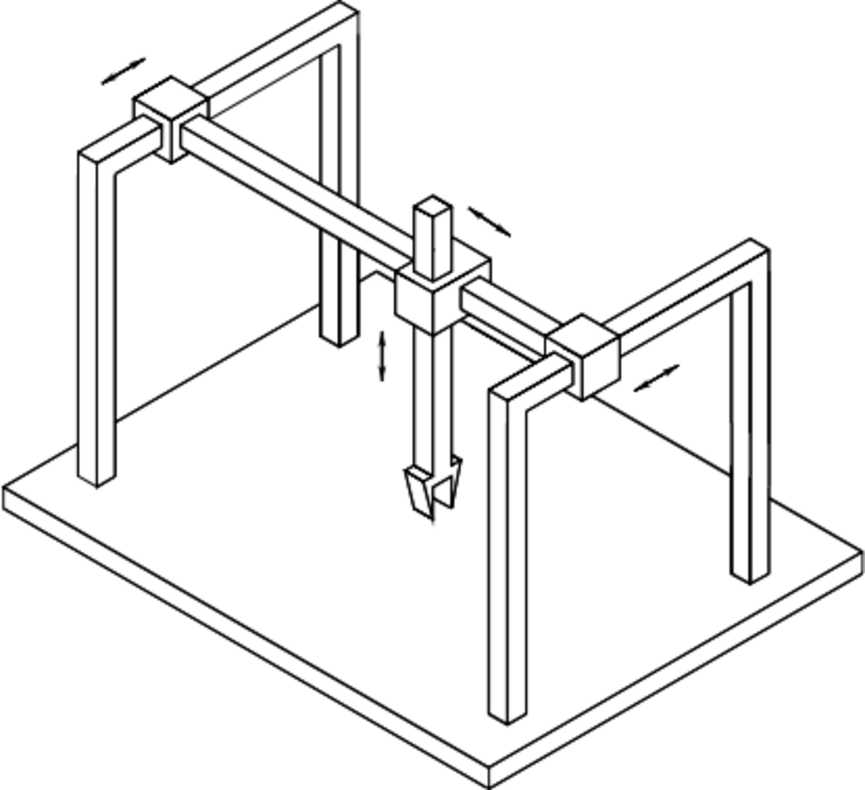
\includegraphics[width=.45\textwidth]{gantry_system_model}
	\hspace{.1in}
	\raisebox{.25\height}{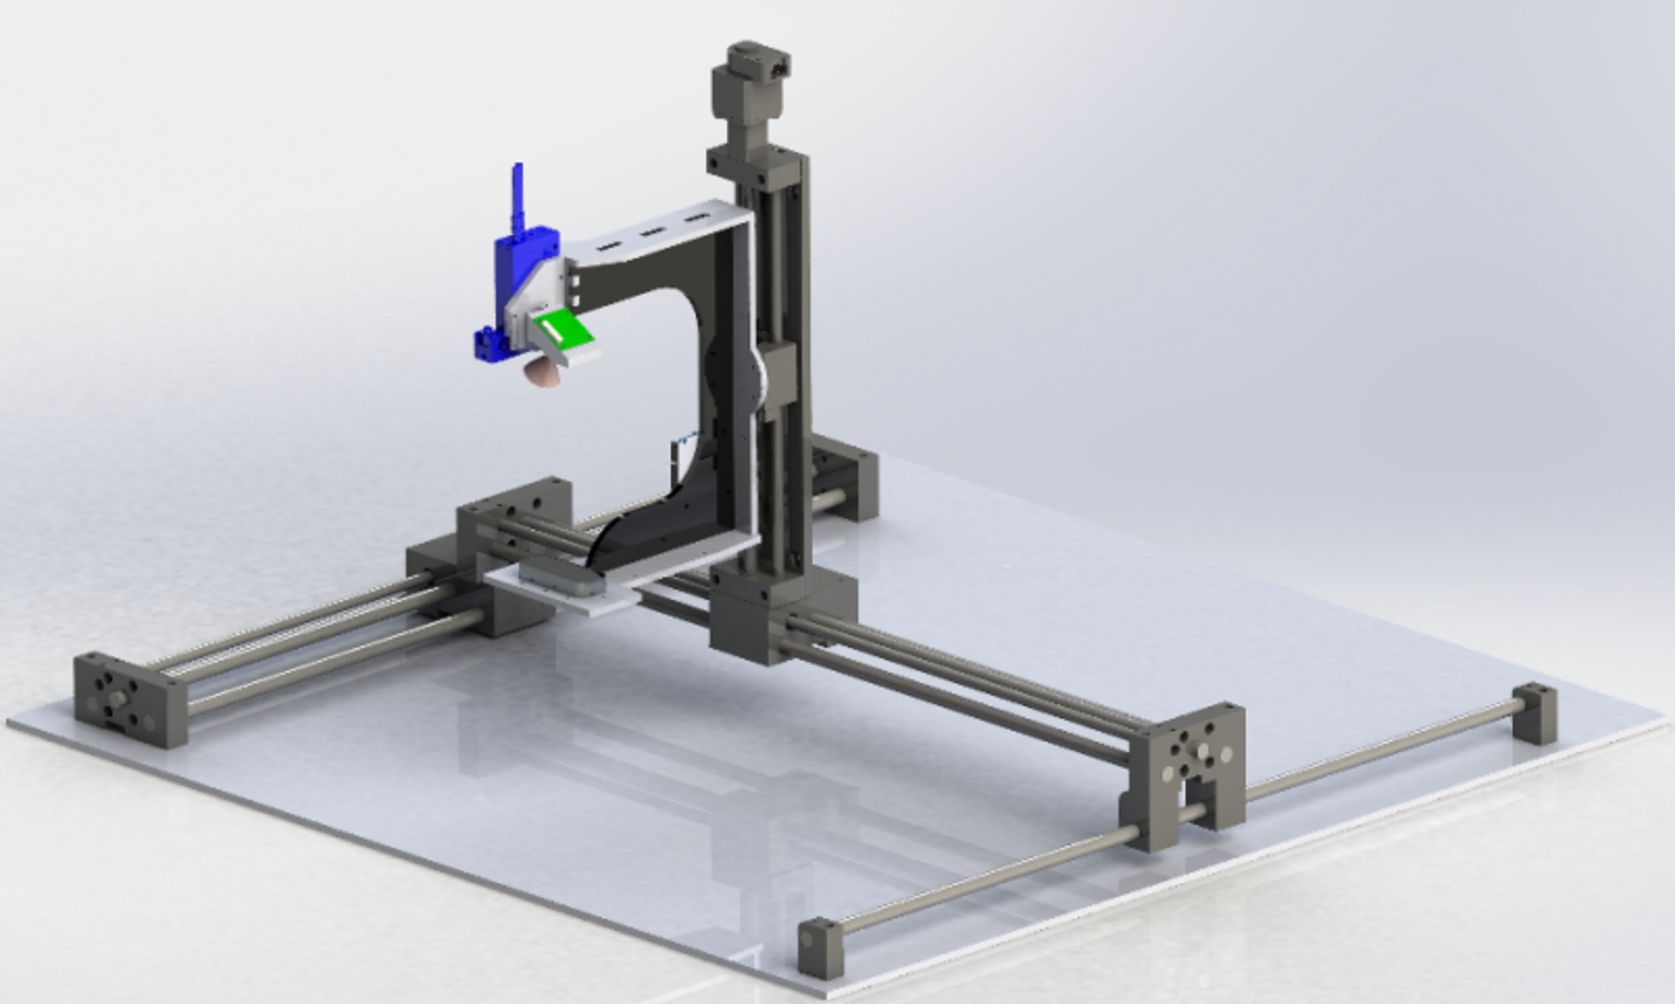
\includegraphics[width=.45\textwidth]{gantry_system_example}}
	\caption[Gantry positioning system.]{Gantry positioning system. (left) System model. Adapted from \cite{Siciliano2009_robotics_modelling_planning_control}. (right) 3D bioprinter example gantry system. Adapted from \cite{ONeill2017_3d_bioprinting_directly_onto_moving_human_anatomy}}
	\label{fig:gantry_system}
\end{figure}

% subsection positioning_system

% = Print head =
\subsection{Print head}
\label{subsec:print_head}

The print head is the bioprinter component responsible for dispensing the bioink. It is the main difference between a 3D bioprinter and a 3D printer.

Some printers have a single print head, while others have two or more. The most common design are single or double print heads. There exists also cases were two robotic arms are used, each one with a print head \cite{Ozbolat2014_multi_arm_bioprinter}. This design concept is useful to improve the printing speed.

However, the most important aspect of the print head is the printing method it uses. Currently, there exists three main printing methods: \gls{lbb}, \gls{dbb}, and \gls{ebb} (Fig. \ref{fig:printing_methods}). The \gls{lbb} and \gls{dbb} methods will be only briefly introduced. The \gls{ebb} will be described more thoroughly because it will be the one used on this thesis.

\begin{figure}[htbp]
	\centering
	\begin{adjustbox}{width=1.2\textwidth,center=\textwidth}
	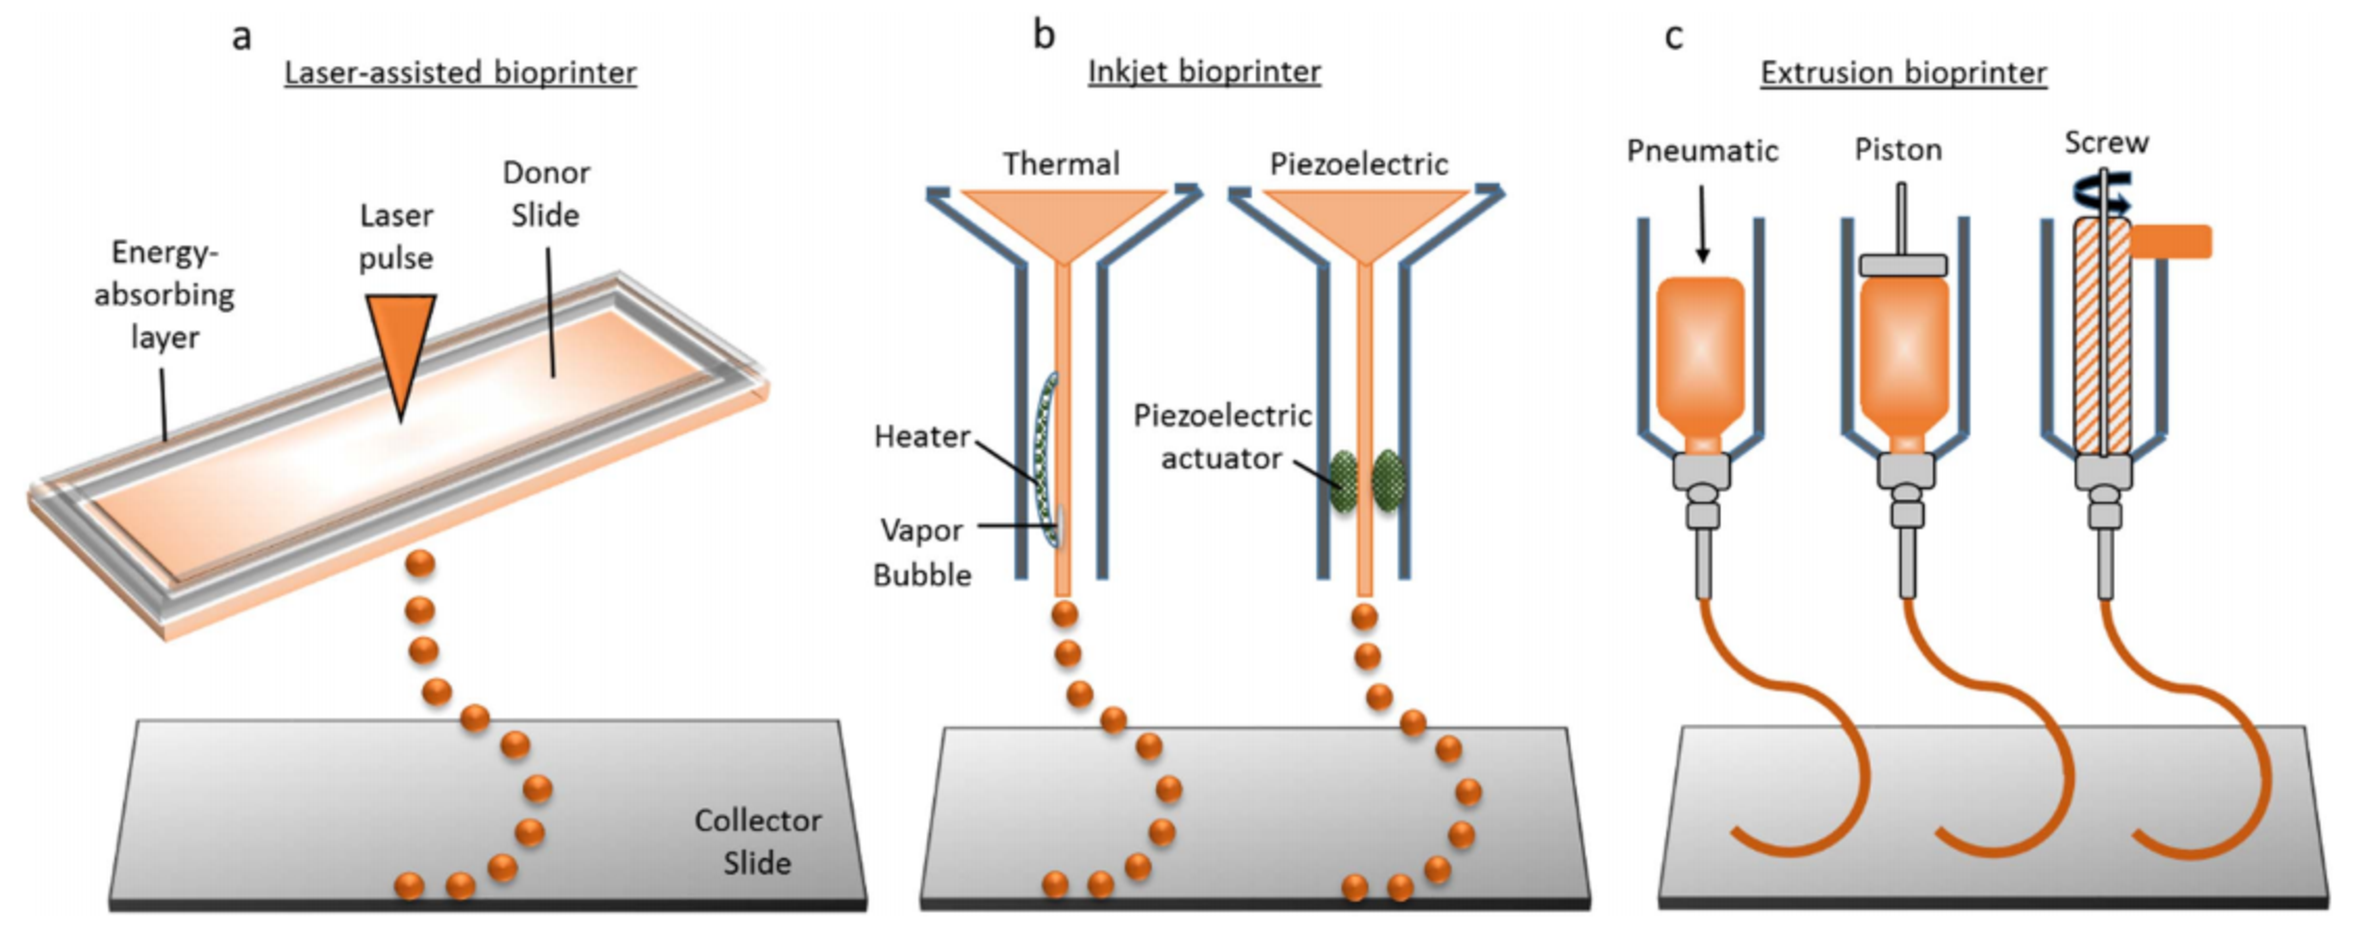
\includegraphics[width=\textwidth]{printing_methods}
	\end{adjustbox}
	\caption[Three main bioprinting technologies.]{Three main bioprinting technologies: (a) Laser-assisted bioprinting focuses laser pulses on to the donor slide, thus creating high pressure to propel droplets of cell-laden hydrogel on to the collector slide; (b) Inkjet printing ejects droplets of biopolymer or cell-laden hydrogels through a nozzle by either thermal energy application (electrically heating to produce vapour bubbles that forces droplets to come out through the nozzle) or piezoelectric actuator (actuation of piezoelectric crystals by applying electrical energy at high frequencies); (c) Extrusion or robotic dispensing bioprinters extrude biopolymers or cell-laden hydrogels through the nozzle by applying air pressure (pneumatic) or mechanical systems (piston or screw). Adapted from \cite{Vijayavenkataraman2016_stateart_modelling_materials_processing}.}
	\label{fig:printing_methods}
\end{figure}


% = Laser-based bioprinting =
\subsubsection{Laser-based bioprinting}
\label{subsubsec:laser_based_bioprinting}

As the name implies, laser-based bioprinting uses laser energy to dispense a bioink on a three dimensional spatial arrangement. It has a high spatial resolution of \numrange{1}{3} \si{\micro\meter}. According to the laser and print ribbon used, the process as slight variations that have different names: LIFT, AFA-LIFT, BioLP, MAPLE DW, and LG DW \cite{Vijayavenkataraman2018_bioprinting_tissues_organs_regen_med}.

\gls{lbb} has several advantages like being a non-contact process, which enables it to have post-printing cell viabilities greater than 95 \%. It also eliminates the nozzle clogging problem. With this method it is possible to print very high cell densities bioinks and low viscosity cell suspensions \cite{Vijayavenkataraman2018_bioprinting_tissues_organs_regen_med}.

% subsubsection laser_based_bioprinting

% = Droplet-based bioprinting =
\subsubsection{Droplet-based bioprinting}
\label{subsubsec:droplet_based_bioprinting}

Droplet-based print heads dispense bioinks in the form of droplets. According to the droplet formation method, \gls{dbb} processes can be classified into inkjet bioprinting, \gls{ehdj}, acoustic bioprinting and microvalve-based bioprinting \cite{Vijayavenkataraman2018_bioprinting_tissues_organs_regen_med}.

Inkjet bioprinting is an adaptation from inkjet printing technology. It can be \gls{cij} or \gls{dod} inkjet printing. Furthermore, \gls{dod} systems can be divided into thermal, piezo-electric or electrostatic, based on the trigger system used \cite{Vijayavenkataraman2018_bioprinting_tissues_organs_regen_med}. This method has several advantages like "high resolution (\textasciitilde 50 \si{\micro\meter}), high printing speed (up to 10,000 droplets per second), affordability, and the ability to introduce cell concentration gradients" \cite{Vijayavenkataraman2018_bioprinting_tissues_organs_regen_med}. Regarding its limitations, inkjet bioprinting can only use low-viscosity bioinks (\textasciitilde \numrange{3}{12} \si{\milli\pascal\second}) and cell concentrations lower than \num{e6} cells \si{\per\milli\litre} because of nozzle clogging \cite{Vijayavenkataraman2018_bioprinting_tissues_organs_regen_med}.

\gls{ehdj} applies a high voltage (\numrange{0.6}{20} \si{\kilo\volt}) "between the nozzle and the substrate as a back-pressure supply delivers the bioink to the nozzle tip" \cite{Vijayavenkataraman2018_bioprinting_tissues_organs_regen_med}. This method's greatest advantage is the high resolution. "A nano-scale resolution of \textasciitilde 100 \si{\nano\meter} had been achieved using this method" \cite{Vijayavenkataraman2018_bioprinting_tissues_organs_regen_med}. It can also bioprint very high viscosity bioinks (up to 20 \% w/v). One limitation is the cell viability on the long-term because of the high voltage applied. Another is the fact that it produces continuous stream of droplets limiting the precision of spatial placement \cite{Vijayavenkataraman2018_bioprinting_tissues_organs_regen_med}.

Acoustic bioprinting can eject bioink droplets on demand using an acoustic actuator. The advantages of this method are high resolution (\textasciitilde 37 \si{\micro\meter}) and high printing speed (up to 10,000 droplets per second). Another advantage is the fact that "the
bioink is in an open pool rather than in a nozzle, thus eliminating the exposure of cells to detrimental stressors such as heat, high pressure, and high voltage" \cite{Vijayavenkataraman2018_bioprinting_tissues_organs_regen_med}.

Microvalve-based bioprinting uses an electromechanical or solenoid valve to control the ejection of bioink droplets. Some limitations of this method are its moderate printing speeds of up to 1000 droplets per second, and nozzle clogging. The nozzle problem is such a challenge that limits the bioink viscosity to a range of \numrange{1}{200} \si{\milli\pascal\second} and a cell concentration less than 106 \si{\per\milli\litre}. Its greatest advantage is the ability of synchronising different print heads, in case multiple are used. This aids "in the printing of co-culture, and multi-culture tissue constructs" \cite{Vijayavenkataraman2018_bioprinting_tissues_organs_regen_med}.

% subsubsection droplet_based_bioprinting

% = Extrusion-based bioprinting =
\subsubsection{Extrusion-based bioprinting}
\label{subsubsec:extrusion_based_bioprinting}

On this method, "the bioink is extruded out of the nozzle using pneumatic pressure or mechanical force by means of a piston or screw" \cite{Vijayavenkataraman2018_bioprinting_tissues_organs_regen_med}. This method is the most widely used, with uses spanning different applications like bioprinting "cells, tissues, organ modules, and organ-on-a-chip devices, for tissue engineering, cancer research, drug testing, and transplantation" \cite{Vijayavenkataraman2018_bioprinting_tissues_organs_regen_med}. The range of tissue types include "bone, cartilage, skeletal muscle, skin, cardiac tissue, nervous tissue, and liver" \cite{Vijayavenkataraman2018_bioprinting_tissues_organs_regen_med}.

Extrusion-based bioprinting has many advantages. The most important one is the scalability. It can print human-scale tissue, "which is impossible with any of the other bioprinting methods" \cite{Vijayavenkataraman2018_bioprinting_tissues_organs_regen_med}. It also works with high viscosity bioinks (\textasciitilde 600 \si{\kilo\pascal\second}) and high cell concentrations, enhancing the printability of natural tissues. In the meanwhile, not everything is perfect. Its resolution is the lowest of all methods (\textasciitilde 100 \si{\micro\meter}). Post-printing cell viability varies from 40 \% to 95 \%, depending on the bioink viscosity, cell concentration and nozzle size. Problems with nozzle clogging is an inherent hurdle of this method. Another limitation is the requirement of "bioinks with shear-thinning property for successful printing, which limits the versatility of the bioinks that could be used" \cite{Vijayavenkataraman2018_bioprinting_tissues_organs_regen_med}.

% subsubsection extrusion_based_bioprinting

% subsection printing_head

% section 3d_bioprinting_systems

% ============
% = Robotics =
% =============

\section{Robotics}
\label{sec:robotics}

There exists many types of robotics systems in use today. On this thesis, the topic of robotics will be restricted to the modelling, planning and control of robotic manipulators.

A robotic manipulator is an electromechanical device composed of a sequence of rigid bodies, or \emph{links}, by means of articulations called \emph{joints}. The mobility of the manipulator is conferred by the number of its joints. At the end of the manipulator a tool can be coupled for a specific task. This tool is also known as the robot \emph{end-effector} \cite{Siciliano2009_robotics_modelling_planning_control}.

To correctly control a robotic manipulator it is important to have a model capable of describing the robot state, movement and dynamics. First, the mathematical tools and concepts necessary to model the robot will be presented. Afterwards, the analysis of robot kinematics, i.e., position and velocity, will be presented. It will be followed by the dynamic model, were forces and torques are considered. The concepts continue through path and trajectory planning, and end with control concepts for free space movement and movement with environment interaction.

The majority of the concepts introduced in this section are based on \cite{Siciliano2009_robotics_modelling_planning_control}. When other sources are used they will be explicitly cited.

% = Rigid motions and homogeneous transformations =
\subsection{Rigid motions and homogeneous transformations}
\label{subsec:rigid_motions_homogeneous_transformations}

The first concept that must be presented is \emph{pose}. Pose is a precise description of a rigid body position and orientation in space, with respect to a reference frame (Fig. \ref{fig:pose_concept}).  

Since a robotic manipulator is a chain of connected rigid bodies, knowing the pose of each link, is important to know the robot state at any time. The main goal regarding the control of robotic manipulators is to control its end-effector. The necessary mathematical concepts to precisely describe the pose of the end-effector are rotation matrices and homogeneous transformations.

\begin{figure}[htbp]
	\centering
	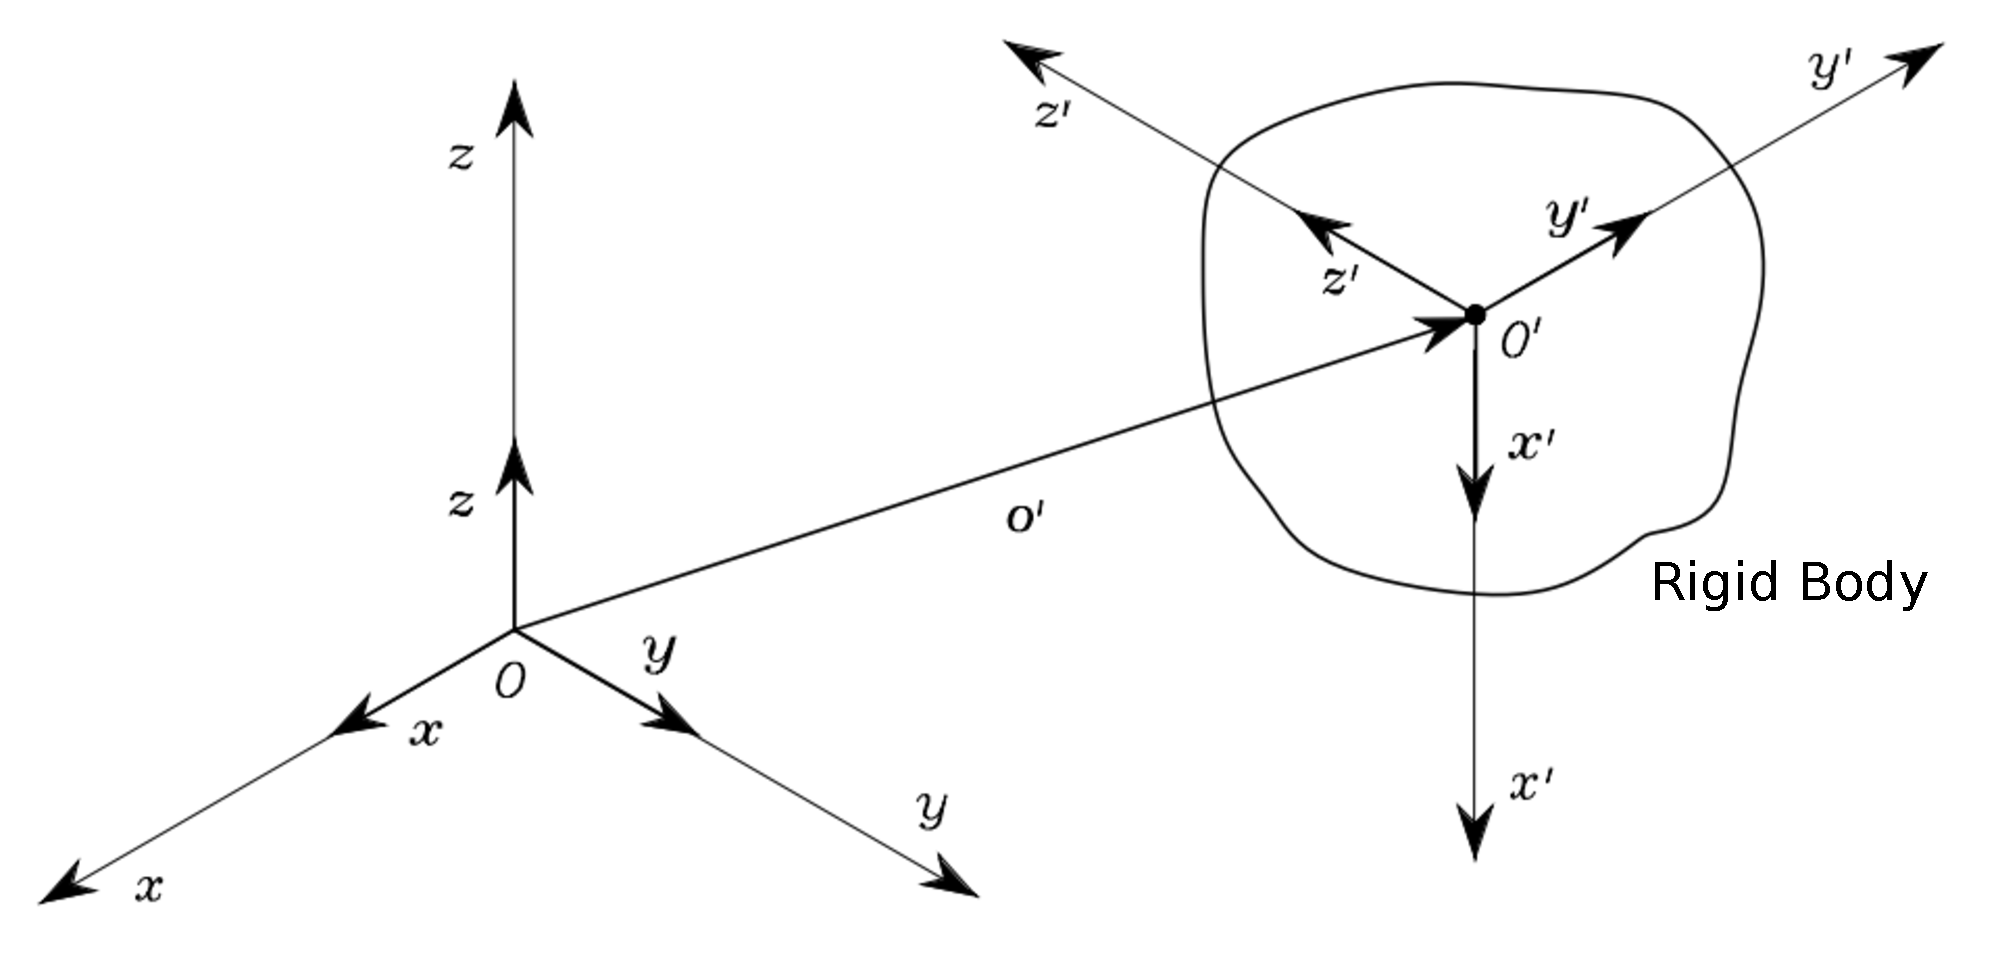
\includegraphics[width=\textwidth]{pose_concept}
	\caption[Concept of Pose.]{Concept of Pose. It consists on the position and orientation of a rigid body in relation to a reference frame. $O-xyz$ is the reference frame and $O^\prime-x^\prime y^\prime z^\prime$ is the rigid body frame. Adapted from \cite{Siciliano2009_robotics_modelling_planning_control}.}
	\label{fig:pose_concept}
\end{figure}

% = Rotation matrices =
\subsubsection{Rotation matrices}
\label{subsubsec:rotation_matrices}

A rotation matrix, is a geometrical tool, heavily used in computer graphics and robotics, that represents the rotation between two different reference frames. On 3D space it is a $3\times3$ matrix, with the columns representing the x, y and z vectors, respectively, of one frame represented on another frame. If $\boldsymbol{R}$ is a rotation matrix then

\begin{equation}
    \boldsymbol{R} = \begin{bmatrix} \boldsymbol{x'} & \boldsymbol{y'} & \boldsymbol{z'}\end{bmatrix} = \begin{bmatrix} r_{11} & r_{12} & r_{13}\\
    r_{21} & r_{22} & r_{23}\\
    r_{31} & r_{32} & r_{33}\end{bmatrix},
\end{equation}

were $\boldsymbol{x'}$, $\boldsymbol{y'}$ and $\boldsymbol{z'}$ are given by

\begin{equation}
    \left\{
    \begin{aligned}
        \boldsymbol{x'} &= x'_x\boldsymbol{x} + x'_y\boldsymbol{y} + x'_z\boldsymbol{z} \\
        \boldsymbol{y'} &= y'_x\boldsymbol{x} + y'_y\boldsymbol{y} + y'_z\boldsymbol{z} \\
        \boldsymbol{z'} &= z'_x\boldsymbol{x} + z'_y\boldsymbol{y} + z'_z\boldsymbol{z}
    \end{aligned}
    \right.
\end{equation}

Rotation matrices are orthogonal, meaning the product between the matrix and its transposed is the identity matrix. This also means that the transpose matrix is equal to the inverse.

\begin{equation}
    \boldsymbol{R}^T \boldsymbol{R} = \boldsymbol{I}_3 \Leftrightarrow \boldsymbol{R}^T = \boldsymbol{R}^{-1}
\end{equation}

The rotation matrices represent general rotations between reference frames. Sometimes it is important to do a rotation just about one of the axis of the main reference frame. These rotations are called \emph{elementary rotations} and represented by $\boldsymbol{R}_{\text{x}}(\alpha)$, $\boldsymbol{R}_{\text{y}}(\alpha)$ and $\boldsymbol{R}_{\text{z}}(\alpha)$. The subscript represents the rotation axis and $\alpha$ is the rotation angle. The matrices are

\begin{equation}
    \boldsymbol{R}_{\text{x}}(\alpha) = 
    \begin{bmatrix} 1 & 0 & 0\\
    0 & \cos{\alpha} & -\sin{\alpha}\\
    0 & \sin{\alpha} & \cos{\alpha}
    \end{bmatrix},
\end{equation}

\begin{equation}
    \boldsymbol{R}_{\text{y}}(\alpha) = \begin{bmatrix} \cos{\alpha} & 0 & \sin{\alpha}\\
    0 & 1 & 0\\
    -\sin{\alpha} & 0 & \cos{\alpha}
    \end{bmatrix},
\end{equation}

\begin{equation}
    \boldsymbol{R}_{\text{z}}(\alpha) = 
    \begin{bmatrix} \cos{\alpha} & -\sin{\alpha} & 0\\
    \sin{\alpha} & \cos{\alpha} & 0\\
    0 & 0 & 1
    \end{bmatrix}.
\end{equation}

Elementary rotations are useful to describe rotations about an arbitrary axis and hold the following properties \cite{Siciliano2009_robotics_modelling_planning_control, Spong2005_robot_dynamics_control} 

\begin{align}
    \boldsymbol{R}_{k}(-\alpha) &= \boldsymbol{R}_{k}^{T}(\alpha) & k = \text{x, y, z}\\
    \boldsymbol{R}_{k}(0) &= \boldsymbol{I}_3 & \\
    \boldsymbol{R}_{k}(\alpha)\boldsymbol{R}_{k}(\beta) &= \boldsymbol{R}_{k}(\alpha+\beta) &
\end{align}

Rotation matrices have three equivalent geometrical meanings \cite{Siciliano2009_robotics_modelling_planning_control}:

\begin{itemize}
    \item They describe "the mutual orientation between two coordinate frames; its column vectors are the direction cosines of the axes of the rotated frame with respect to the original frame".
    \item They represent "the coordinate transformation between the coordinates of a point expressed in two different frames (with common origin)".
    \item They are "the operator that allows the rotation of a vector in the same coordinate frame".
\end{itemize}

Another important aspect of rotation matrices is the fact that they can be combined in order to represent complex rotations. Considering that $\boldsymbol{R}^{i}_{j}$ represents the rotation of reference frame $j$ in relation to reference $i$, rotation matrices composition is given by

\begin{equation}
    \boldsymbol{R}^{0}_{2} = \boldsymbol{R}^{0}_{1}\boldsymbol{R}^{1}_{2}
\end{equation}

if the rotation are in relation to the \emph{current frame}, or

\begin{equation}
    \boldsymbol{R}^{0}_{2} = \boldsymbol{R}^{1}_{2}\boldsymbol{R}^{0}_{1}
\end{equation}

if they are in relation to a fixed frame.

Finally, sometimes its is convenient to use a simplified representation of rotations based on less parameters. There exist four representations commonly used:

\begin{itemize}
    \item Euler angles
    \item Roll, Pitch, Yaw
    \item Axis/Angle
    \item Unit Quaternion
\end{itemize}

% subsubsection rotation_matrices

% = Homogeneous transformations =
\subsubsection{Homogeneous transformations}
\label{subsubsec:homogeneous_transformations}

To properly represent the position and orientation of a rigid body we use the pose. But we also need to represent a pose change given by a translation, a rotation or a combination of both. The mathematical tool to represent this change in pose is a $4\times4$ matrix, in 3D space, called homogeneous transformation. This matrix, represented by $\boldsymbol{H}$ in (\ref{eq:homogeneous_transformation}), is composed by a rotation matrix and a translation vector that describe the pose.

\begin{equation}
    \label{eq:homogeneous_transformation}
    \boldsymbol{H} = \begin{bmatrix} \boldsymbol{R} & \boldsymbol{p} \\ 
    \boldsymbol{0}^{T} & 1\end{bmatrix} = \begin{bmatrix} r_{11} & r_{12} & r_{13} & p_x\\
    r_{21} & r_{22} & r_{23} & p_y\\
    r_{31} & r_{32} & r_{33} & p_z\\
    0 & 0 & 0 & 1\end{bmatrix}
\end{equation}

In general, the homogeneous transformation matrix is not orthogonal so 
\begin{equation}
    \boldsymbol{H}^{T} \neq \boldsymbol{H}^{-1}.
\end{equation}

Homogeneous transformations follow the some composition rules of rotations matrices. Considering that $\boldsymbol{H}^{i}_{j}$ represents the homogeneous transformation of reference frame $j$ in relation to reference $i$, the composition is given by

\begin{equation}
    \boldsymbol{H}^{0}_{2} = \boldsymbol{H}^{0}_{1}\boldsymbol{H}^{1}_{2}
\end{equation}

if the transformations are in relation to the \emph{current frame}, or

\begin{equation}
    \boldsymbol{H}^{0}_{2} = \boldsymbol{H}^{1}_{2}\boldsymbol{H}^{0}_{1}
\end{equation}

if they are in relation to a fixed frame.

% subsubsection Homogeneous transformations

% subsection rigid_motions_homogeneous_transformations

% = Kinematics =
\subsection{Kinematics}
\label{subsec:kinematics}

The study of robot kinematics is fundamental to understand how a robotic manipulator moves in space. Kinematics study is divided into three branches: (a) Direct or \gls{fk}; (b) \gls{ik}; and (c) Differential Kinematics.\bigskip

Before we jump on to the different branches it is important to introduce a few other concepts about manipulators. A manipulator is considered to be an \emph{open chain} from the kinematic point-of-view if there is only a single sequence of links connecting the base link to the end-effector. We have a \emph{closed chain} when a sequence of links form a loop. The robot joints can be \emph{revolute} or \emph{prismatic} when the movement between consecutive links is rotational or translational, respectively. The robot \emph{posture}, or the pose of all the links, is mecanically defined by a number of degrees-of-freedom (\gls{dof}). Each \gls{dof} is associated to a robot joint and represents a \emph{joint variable}.

% = Forward Kinematics =
\subsubsection{Forward kinematics}
\label{subsubsec:forward_kinematics}

The goal of forward kinematics is to find the pose of the end-effector according to the state of the joint variables.

Mathematically, its is represented by the homogeneous transformation of the \emph{end-effector frame}, $O_{\text{e}}x_{\text{e}}y_{\text{e}}z_{\text{e}}$, in relation to the \emph{base frame}, $O_{\text{b}}x_{\text{b}}y_{\text{b}}z_{\text{b}}$, $\boldsymbol{H}^{\text{b}}_{\text{e}}$. 

\begin{equation}
    \boldsymbol{H}^{\text{b}}_{\text{e}}(\boldsymbol{q}) =
    \begin{bmatrix}
    \boldsymbol{n}^{\text{b}}_{\text{e}}(\boldsymbol{q}) & \boldsymbol{s}^{\text{b}}_{\text{e}}(\boldsymbol{q}) & \boldsymbol{a}^{\text{b}}_{\text{e}}(\boldsymbol{q}) & \boldsymbol{p}^{\text{b}}_{\text{e}}(\boldsymbol{q})\\
    0 & 0 & 0 & 1
    \end{bmatrix},
\end{equation}

where $\boldsymbol{q}$ is the vector of the joint variables, $\boldsymbol{n}_{\text{e}}$, $\boldsymbol{s}_{\text{e}}$, $\boldsymbol{a}_{\text{e}}$ are the unit vectors that form the end-effector frame, and $\boldsymbol{p}_{\text{e}}$ is the position vector of the end-effector frame origin.

This open chain homogeneous transformation (\ref{eq:homogeneous_transformation_b_e}) is a composition of homegeneous transformations between consecutive frames attached to each link and end-effector.

\begin{align}
    \label{eq:homogeneous_transformation_b_e}
    \boldsymbol{H}^{\text{b}}_{\text{e}}(\boldsymbol{q}) &= \boldsymbol{H}^{\text{b}}_{\text{0}}\boldsymbol{H}^{\text{0}}_{\text{n}}(\boldsymbol{q})\boldsymbol{H}^{\text{n}}_{\text{e}} \\
    \boldsymbol{H}^{\text{0}}_{\text{n}}(\boldsymbol{q}) &= \boldsymbol{H}^{\text{0}}_{\text{1}}(q_1)\boldsymbol{H}^{\text{1}}_{\text{2}}(q_2)\boldsymbol{H}^{\text{2}}_{\text{3}}(q_3)\ldots\boldsymbol{H}^{\text{n-1}}_{\text{n}}(q_n)
\end{align}

$\boldsymbol{H}^{\text{b}}_{\text{0}}$ and $\boldsymbol{H}^{\text{n}}_{\text{e}}$ represent transformations between the first chain link and the base frame, and the last chain link and the end-effector frame, respectively. These two transformations are typically constant.

Although equation (\ref{eq:homogeneous_transformation_b_e}) mathematically defines the way to compute the transformation between the end-effector frame and the base frame, the actual process is highly dependent on the way the reference frames for each link are defined. Because there is freedom on the choice of the reference frames, sometimes the process becomes too laborious when the choice is not convenient. Taking this into consideration the \glsfirst{dh} convention was created. This convention defines a systematic approach to the process of choosing the reference frames. Despite that fact that it eases the process, it still does not present a unique solution. It is possible to have various different reference frame choices still valid according to the \gls{dh} rules.

Following the \gls{dh} convention, the homogeneous transformation between consecutive links is given by (\ref{eq:homogeneous_transformation_dh}).

\begin{equation}
    \label{eq:homogeneous_transformation_dh}
    \boldsymbol{H}^{i-1}_{i}(q_i) = \begin{bmatrix}
        c_{\theta_i} & -s_{\theta_i}c_{\alpha_i} & s_{\theta_i}s_{\alpha_i} & a_{i}c_{\theta_i}\\
        s_{\theta_i} & c_{\theta_i}c_{\alpha_i} & -c_{\theta_i}s_{\alpha_i} & a_{i}s_{\theta_i}\\
        0 & s_{\alpha_i} & c_{\alpha_i} & d_{i}\\
        0 & 0 & 0 & 1
    \end{bmatrix}
\end{equation}

$c_k$ and $s_k$ represent, respectively, the cosine of $k$ and the sine of $k$. The variables $\theta_i$, $\alpha_i$, $d_i$ and $a_i$ are the \gls{dh} parameters that define the relation between links $i-1$ and $i$. The meaning of these parameters are defined as (see Fig. \ref{fig:dh_parameters}) \cite{Siciliano2009_robotics_modelling_planning_control}:

\begin{itemize}
    \item $a_i$ distance between the reference frames origins, $O_i$ and $O_{i'}$.
    \item $d_i$ coordinate of $O_{i'}$ along $z_{i-1}$
    \item $\alpha_i$ angle between axes $z_{i-1}$ and $z_i$ about axis $x_i$ to be taken positive when rotation is made counter-clockwise.
    \item $\theta_i$ angle between axes $x_{i-1}$ and $x_i$ about axis $z_{i-1}$ to be taken positive when rotation is made counter-clockwise.
\end{itemize}

\begin{figure}[htbp]
	\centering
	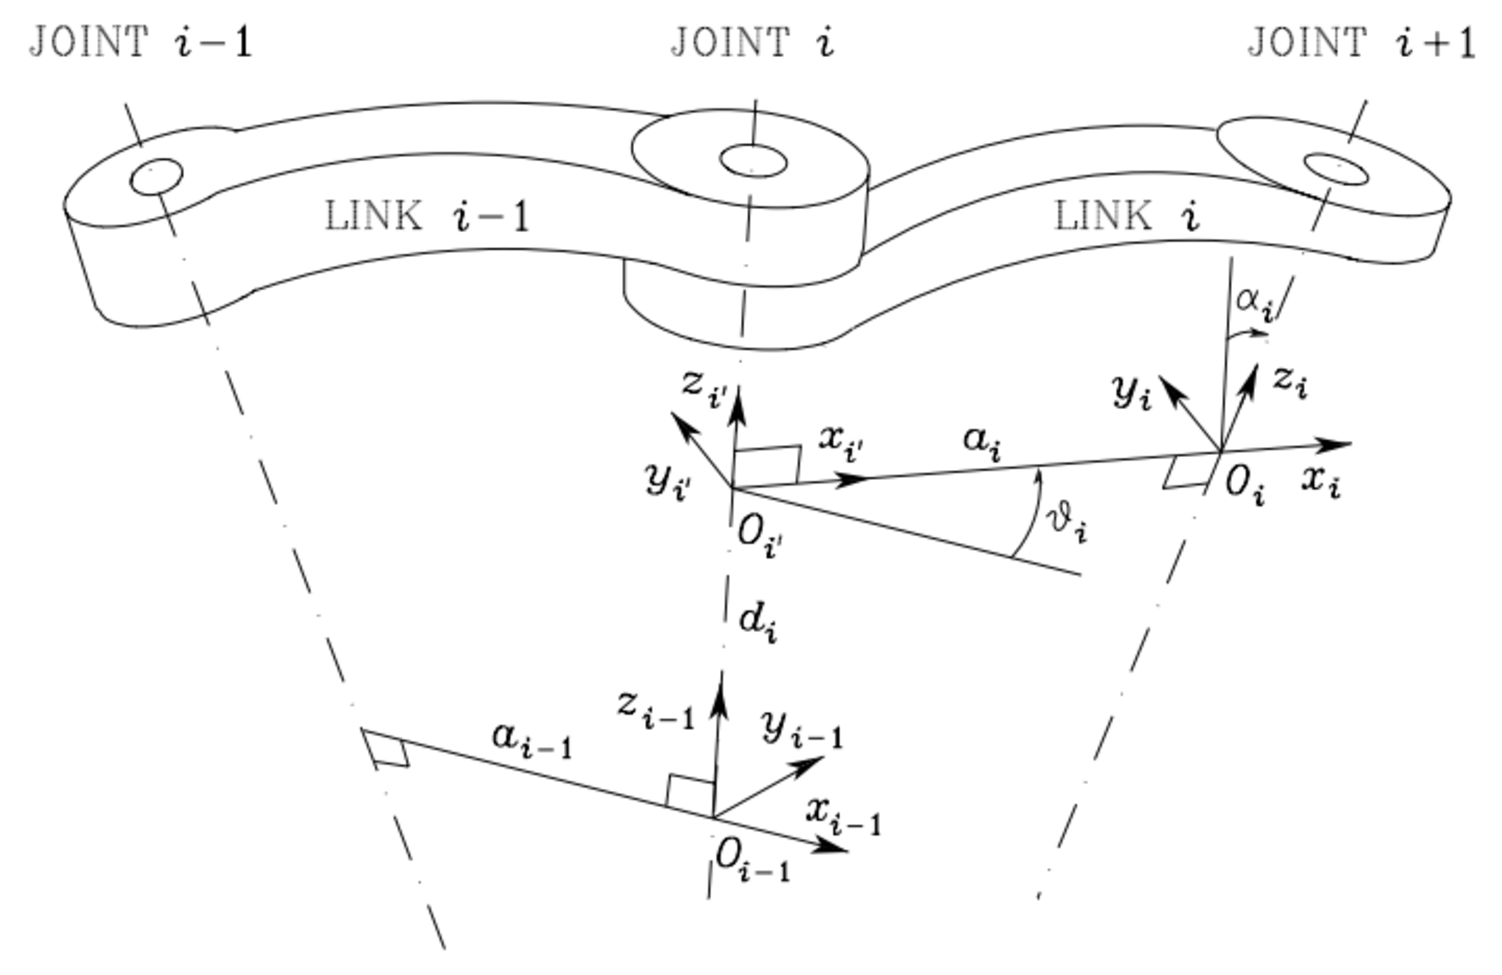
\includegraphics[width=\textwidth]{dh_parameters}
	\caption[Denavit-Hartenberg kinematic parameters.]{Denavit-Hartenberg kinematic parameters. Adapted from \cite{Siciliano2009_robotics_modelling_planning_control}.}
	\label{fig:dh_parameters}
\end{figure}

% subsubsection forward_kinematics

% = Differential Kinematics =
\subsubsection{Differential kinematics}
\label{subsubsec:differential_kinematics}

Differential kinematics establishes the relation between joint velocities and end-effector linear and angular velocities. The mapping between velocities described by a matrix, \emph{geometric jacobian}, or jacobian for short. This matrix depends on the posture of the robot. The jacobian matrix is a very important tool to characterise a robotic manipulator. Some examples of its application are to find \emph{singularities}, analyse \emph{redundancy}, for inverse kinematics, and to relate joint torques to end-effector forces.

Defining $\boldsymbol{v}_e$ as the end-effector velocity, the jacobian is defined by the following equation

\begin{equation}
    \boldsymbol{v}_e = \begin{bmatrix}
    \dot{\boldsymbol{p}}_e\\
    \boldsymbol{\omega}_e
    \end{bmatrix} = \boldsymbol{J}(\boldsymbol{q})\dot{\boldsymbol{q}}.
\end{equation}

The matrix $\boldsymbol{J}$ is the manipulator jacobian and is a $6 \times n$ matrix, where $n$ is the number of joints. The jacobian can be defined as being composed of two jacobians, the linear jacobian $\boldsymbol{J}_\text{P}$, and the angular jacobian $\boldsymbol{J}_\text{O}$, like

\begin{equation}
    \boldsymbol{J} = \begin{bmatrix}
    \boldsymbol{J}_\text{P}\\
    \boldsymbol{J}_\text{O}
    \end{bmatrix}.
\end{equation}

In general, the jacobian can be partitioned into column vectors ($3\times1$), $\boldsymbol{J}_{\text{P}i}$ and $\boldsymbol{J}_{\text{O}i}$ as

\begin{equation}
    \boldsymbol{J} = \begin{bmatrix}
    \boldsymbol{J}_{\text{P}1} & \ldots & \boldsymbol{J}_{\text{P}n} \\
    \boldsymbol{J}_{\text{O}1} & \ldots & \boldsymbol{J}_{\text{O}n}
    \end{bmatrix},
\end{equation}

where each column is defined as

\begin{equation}
    \label{eq:jacobian_column}
    \boldsymbol{J} = \begin{bmatrix}
    \boldsymbol{J}_{\text{P}i}\\
    \boldsymbol{J}_{\text{O}i}
    \end{bmatrix} = \left\{ \begin{array}{cc}
        \begin{bmatrix}
            \boldsymbol{z}_{i-1}\\
            \boldsymbol{0}
        \end{bmatrix} & \text{for prismatic joint} \\
        \begin{bmatrix}
        \boldsymbol{z}_{i-1} \times (\boldsymbol{p}_\text{e} - \boldsymbol{p}_{i-1})\\
        \boldsymbol{z}_{i-1}
        \end{bmatrix} & \text{for revolute joint}.
    \end{array}\right.
\end{equation}

Using only the relations from \gls{fk} and the expressions in (\ref{eq:jacobian_column}) the jacobian is easily computed.

% subsubsection differential_kinematics

% subsection kinematics

% = Dynamics =
\subsection{Dynamics}
\label{subsec:dynamics}

The study of the robot dynamics is concerned with the analysis of motion taking into consideration the forces and moments that generate that motion. The robotic manipulator's equations of motion will be introduced from the \gls{el} equations. These concepts follow the notation from \cite{Spong2005_robot_dynamics_control}.

The \gls{el} equations are defined as

\begin{equation}
    \label{eq:euler_lagrange_equations}
    \frac{d}{dt}\frac{\partial L}{\partial\dot{q}_j}-\frac{\partial L}{\partial q_j} = \tau_j ,
\end{equation}

\begin{equation}
    L = K - P,
\end{equation}

where $L$ is the Lagrangian and $K$ and $P$ are the kinetic and potential energies, respectively. The variables $\dot{q}_j$, $q_j$ and $\tau_j$ represent, respectively, the $j$-th joint's velocity, displacement and torque.

For an $n$-link robot manipulator, the kinetic and potential energies are defined as followed:

\begin{equation}
    \label{eq:kinetic_energy}
    K = \frac{1}{2}\dot{\boldsymbol{q}}^T M(\boldsymbol{q}) \dot{\boldsymbol{q}},
\end{equation}

\begin{equation}
    \label{eq:potential_energy}
    P = \sum^{n}_{i=1} P_i = \sum^{n}_{i=1} \boldsymbol{g}^T \boldsymbol{r}_{\text{c}i} m_i .
\end{equation}

On the definition of the kinetic energy, $M(\boldsymbol{q})$ is the \emph{inertia matrix}, which is a positive definite matrix dependent on the robot configuration. $\dot{\boldsymbol{q}}$ is the vector of the joint velocities.
The potential energy is a function of the gravity vector, $\boldsymbol{g}$, the center of mass vectors for each link, $\boldsymbol{r}_{\text{c}i}$, and the links mass $m_i$.

By substituting the kinetic (\ref{eq:kinetic_energy}) and potential (\ref{eq:potential_energy}) energies on the \gls{el} equations (\ref{eq:euler_lagrange_equations}), and applying some algebraic operations, we obtain the robotic manipulator equations of motion. These equations in matrix form are defined as

\begin{equation}
    \label{eq:equations_motion}
    M(\boldsymbol{q})\ddot{\boldsymbol{q}} + C(\boldsymbol{q}, \dot{\boldsymbol{q}})\dot{\boldsymbol{q}} + \boldsymbol{g}(\boldsymbol{q}) = \boldsymbol{\tau}.
\end{equation}

$C(\boldsymbol{q}, \dot{\boldsymbol{q}})$ is a $n \times n$ matrix, with \emph{centrifugal} and \emph{Coriolis} terms. Its $k$,$j$-th element is defined as

\begin{align}
    c_{kj} &= \sum^n_{i=1} c_{ijk}(\boldsymbol{q})\dot{q}_i \\
    &= \sum^n_{i=1} \frac{1}{2} \left\{ \frac{\partial d_{kj}}{\partial q_j} + \frac{\partial d_{ki}}{\partial q_j} - \frac{\partial d_{ij}}{\partial q_k} \right\}.
\end{align}

The terms $c_{ijk}$ are known as the \emph{Christoffel symbols} of the first kind.

% subsection dynamics

% = Path and trajectory planning =
\subsection{Path and trajectory planning}
\label{subsec:path_trajectory_planning}

The execution of a robot task is normally associated with movement of the end-effector in space. For proper and safe execution of the movements, obstacle avoidance and the application of the right velocities and accelerations must be considered. For this, path and trajectory planning are essential.

A path consists of the points in space that the robot should occupy while executing the task. A trajectory, associates a timing law to a path, i.e., it defines velocities and accelerations. It defines how the robot should move from the start to the end of the path.

The main goal of path and trajectory planning is to guarantee that the robot does not violate its physical limits during the task execution. This planning can be done on the \emph{configuration space} or the \emph{operational space}. The configuration space is the space defined by the joint variables. The operational or task space is defined by the task \gls{dof}, generally, a six dimensional space (three for position and three for orientation).

% = Joint space trajectories =
\subsubsection{Joint space trajectories}
\label{subsubsec:joint_space_trajectories}

Joint space trajectory planning is the most efficient on guaranteeing that the robot stays within its own limits. It is intended that the robot executes smooth trajectories, meaning that the velocities and accelerations are continuous functions. There exist several functions that guarantee this continuity. In order to interpolate between two path points, the most simple and common function used is a 3rd degree polynomial.

If $q(t)$ represents a single joint motion in time, the cubic polynomial that defines it is

\begin{equation}
    q(t) = a_3 t^3 + a_2 t^2 + a_1 t + a_0 \text{.}
\end{equation}

This trajectory will originate a parabolic velocity profile

\begin{equation}
    \dot{q}(t) = 3 a_3 t^2 + 2 a_2 t + a_1\text{,}
\end{equation}

and a linear acceleration profile

\begin{equation}
    \ddot{q}(t) = 6 a_3 t + 2 a_2\text{.}
\end{equation}

Figure \ref{fig:cubic_trajectory_planning} shows the timing law for position, velocity and acceleration for the cubic polynomial.

Since four coefficients are available, it is possible to impose the initial and final positions and velocities (\ref{eq:cubic_polynomial_coefficients}). Typically the initial and final velocities are chosen to be zero.

\begin{equation}
    \label{eq:cubic_polynomial_coefficients}
    \begin{aligned}
        a_0 &= q_i\\
        a_1 &= \dot{q}_i \\
        a_3 t_f^3 + a_2 t_f^2 + a_1 t + a_0 &= q_f \\
        3 a_3 t_f^2 + 2 a_2 t_f + a_1 &= \dot{q}_f 
    \end{aligned}
\end{equation}

\begin{figure}[htbp]
	\centering
	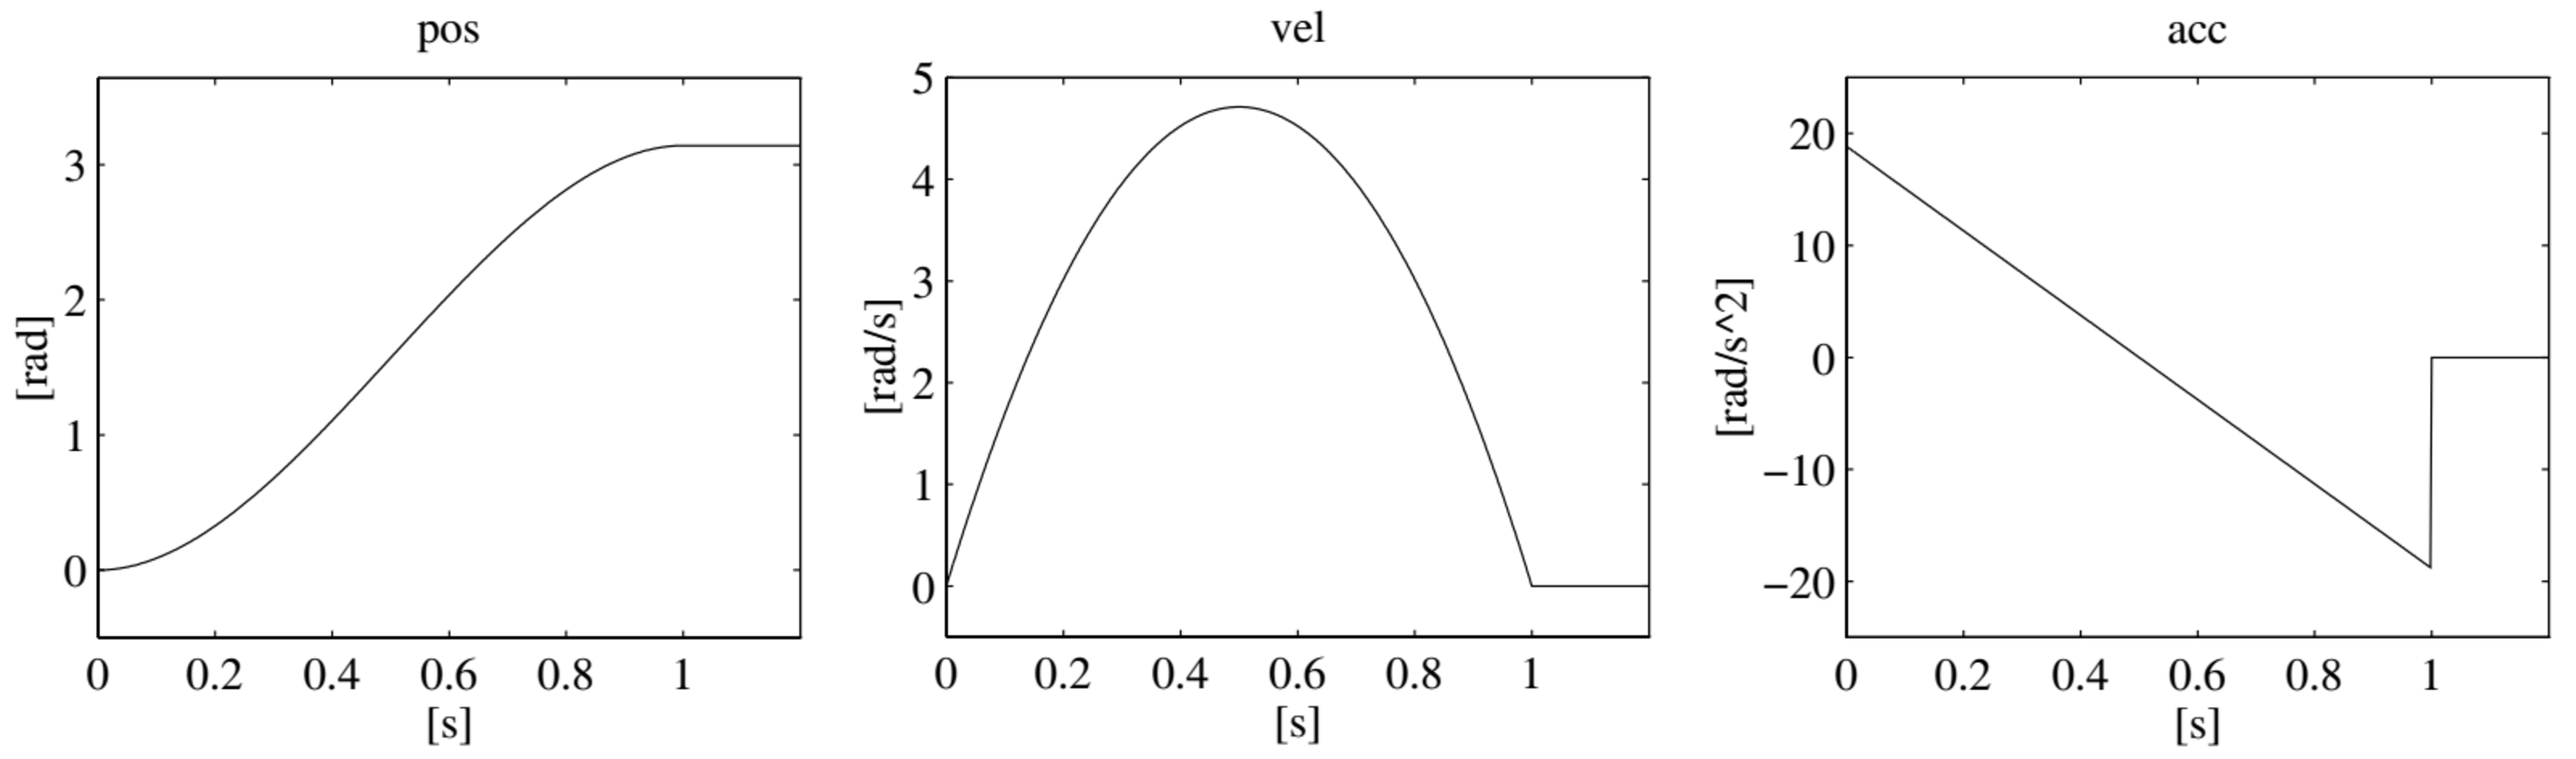
\includegraphics[width=\textwidth]{cubic_trajectory_planning}
	\caption[Time history of position, velocity and acceleration with a cubic polynomial timing law.]{Time history of position, velocity and acceleration with a cubic polynomial timing law. Adapted from \cite{Siciliano2009_robotics_modelling_planning_control}}
	\label{fig:cubic_trajectory_planning}
\end{figure}

% subsubsection joint_space_trajectories

% = Task space trajectories =
\subsubsection{Task space trajectories}
\label{subsubsec:task_space_trajectories}

Configuration space trajectories strategies are effective to guarantee a smooth trajectory between two different robot configurations. However, with this approach it is not easy to predicte the end-effector movement. Because most of the times the task is related to the end-effector position and movement, it is important to be able to plan a trajectory explicitly for the end-effector \cite{Siciliano2009_robotics_modelling_planning_control}.

As in the case of joint space trajectories, the planning must generate some trajectories of the end-effector. On a point-to-point approach, the trajectory is an interpolation of the robot pose between an initial and a final pose.

The rational can be used for task space trajectories. It means that we can also use a cubic polynomial to represent the 6 degrees of freedom of the end-effector (\ref{eq:cubic_polynomial_coefficients_task_space}). An important note is that, to interpolate the orientation a parametric representation must be used, like axis/angle or unit quaternion.

\begin{equation}
    \label{eq:cubic_polynomial_coefficients_task_space}
    \boldsymbol{X}(t) = \left\{
    \begin{aligned}
        x(t) &= a_3 t^3 + a_2 t^2 + a_1 t + a_0\\
        y(t) &= b_3 t^3 + b_2 t^2 + b_1 t + b_0\\
        z(t) &= c_3 t^3 + c_2 t^2 + c_1 t + c_0\\
        rx(t) &= e_3 t^3 + e_2 t^2 + e_1 t + e_0\\
        ry(t) &= f_3 t^3 + f_2 t^2 + f_1 t + f_0\\
        rz(t) &= g_3 t^3 + g_2 t^2 + g_1 t + g_0
    \end{aligned}
    \right.
\end{equation}

The notation used for orientation is axis/angle. The trajectory time is equal for each degree of freedom.

% subsubsection task_space_trajectories

% subsection path_trajectory_planning

% = Free space and interaction control =
\subsection{Free space and interaction control}
\label{subsec:free_space_interaction_control}

After the trajectories are planned, the robot must execute them and evaluate or track the execution. This is the responsibility of the control algorithm.

Robot control is part of general control theory. Control algorithms are vital for many different type of systems, from airplanes to air conditioning systems. The control can be done in \emph{open-loop} or \emph{close-loop}. Open-loop control inputs a control signal to the system, but does not observe the system's output. It is a \emph{fire-and-forget} type of control. On the contrary, close-loop control has a feedback system where the system's output is combined with the control signal. This new signal affects the system in order for it to asymptotically reach the desired state.\\  

On the case of robot manipulators, control can be related to free space motion (\emph{motion control}) or robot interaction with the environment (\emph{interaction control}) \cite{Siciliano1999_robot_force_control}. 

Motion control should only be used on a task where the robot is moving in free space. If this approach is used when the robot is in interaction with environment, a small tracking error can lead to high forces and eventually damage to the robot and/or environment. 

Interaction control was especially conceived to deal with interactions forces from the environment. This control also subdivides into {indirect force control} and {direct force control}. The difference between the two, is that the former achieves force control via motion control. The latter controls the contact force directly \cite{Siciliano1999_robot_force_control}.

% subsection free_space_interaction_control

% section robotics

% ===================
% = Computer Vision =
% ===================

\section{Computer vision}
\label{sec:computer_vision}

Computer vision is a branch of computer science that has as goal to be able to mimic the human visual capabilities. This means acquiring visual data and infer or extract information from it. It is a very broad area that deals with the hardware side of image/video/depth acquisition systems, and also the software side with the algorithms for information extraction.

For the scope of this thesis, it is important to present some concepts about: (a) digital image data format; (b) image segmentation algorithms; (c) the hardware necessary to extract depth data; and (d) the format of depth data itself.

% = Digital Image =
\subsection{Digital Image}
\label{subsec:digital_image}

An image is a 2D visual representation of a scene or concept. It is composed of several colours or a single colour. An example is a drawing or a painting.

With the development of computer screens it became important to represent images digitally. A digital image is represented by a matrix, $I$, where each cell is called a pixel (\ref{eq:image_matrix_representation}). Each pixel stores a number that represents the light intensity captured by a light sensible device, or produced by a computer system.

\begin{equation}
    \label{eq:image_matrix_representation}
    I(x, y) = \begin{bmatrix}
        i_{11} && i_{12} && {}\ldots{} && i_{1w} \\
        i_{21} && i_{22} && {}\ldots{} && i_{2w} \\
        \vdots && \vdots  && \vdots  && \vdots \\
        i_{h1} && i_{h2} && {}\ldots{} && i_{hw}\\
    \end{bmatrix}
\end{equation}

where $i_{xy} \in Y$. $Y$ represents a set of numbers that depends on the image data type. The data type defines the intensity gradation. For example, a \textit{uint8} representation has 256 different intensity values, from 0 to 255.

The number of columns and rows of the matrix $I$ represent the image width (W) and height (H), respectively. These dimensions define the image resolution (Fig. \ref{fig:image_matrix}).\\

\begin{figure}[htbp]
	\centering
	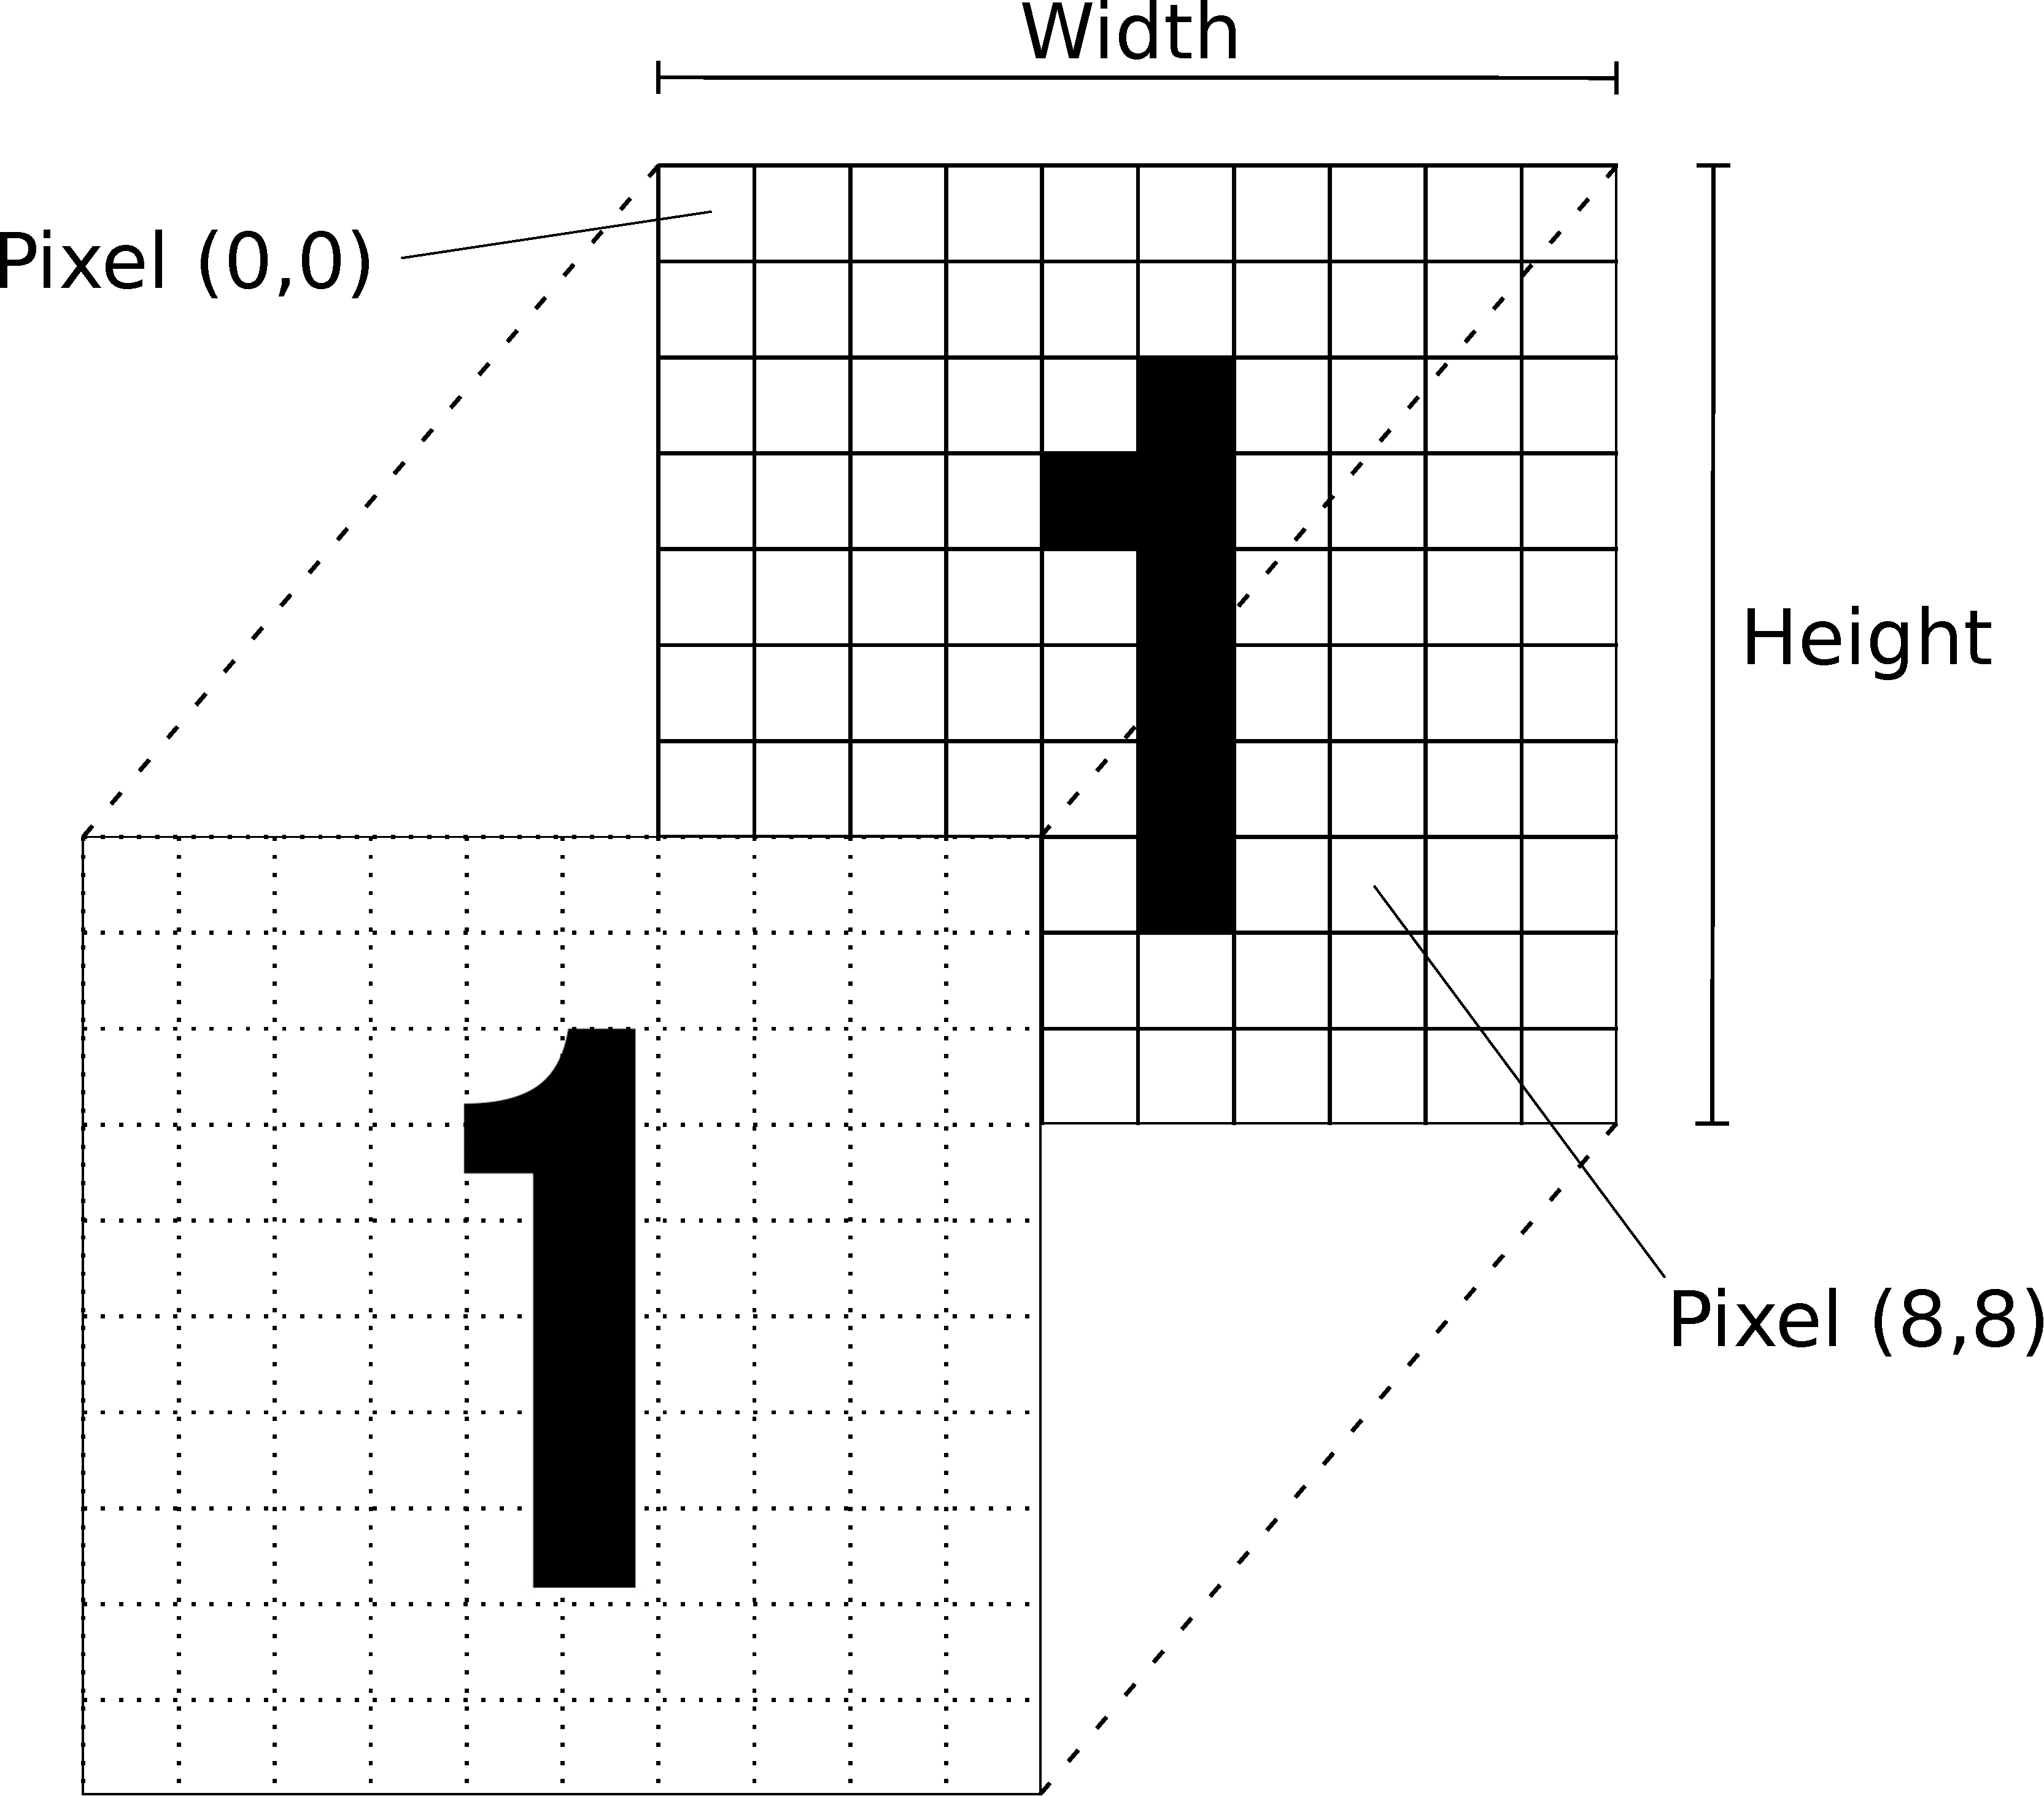
\includegraphics[width=.7\textwidth]{image_matrix}
	\caption[Digital image matrix representation.]{Digital image matrix representation.}
	\label{fig:image_matrix}
\end{figure}

An image can have different colour spaces. The three main ones are: binary, grayscale, and \gls{rgb} (Fig. \ref{fig:image_binary_grayscale_rgb}). On a binary image, each pixel can only assume two values, either 0 or 1. The value zero represents a black pixel and 1 a white pixel. A grayscale image already as a tone gradation. It goes from black all the way to white, passing by various tones of grey with increasing brightness. An \gls{rgb} image has a major difference between the other two. It has three channels instead of one (\ref{eq:rgb_image_matrix}). Each channel represents the intensity of a colour: red, green or blue. The combination of intensities of each channel defines the colour of each pixel.

\begin{figure}[htbp]
	\centering
	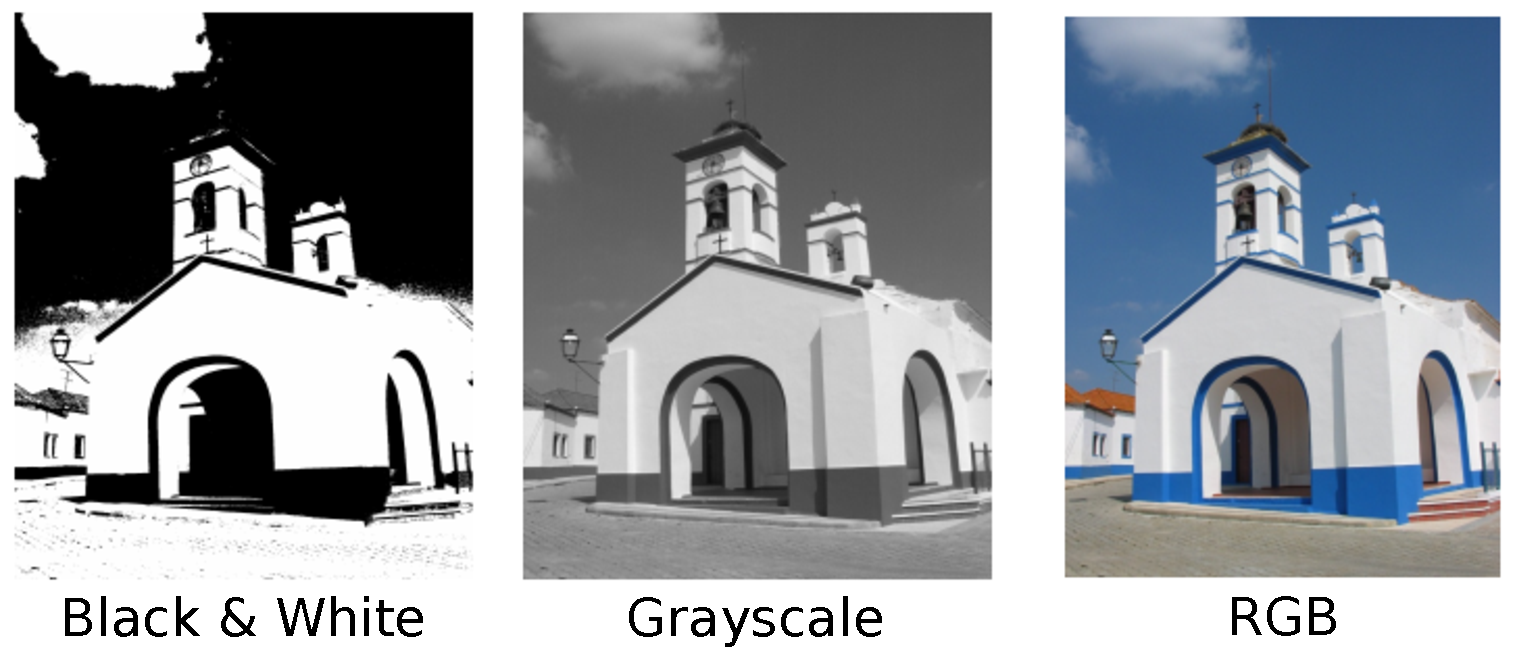
\includegraphics[width=\textwidth]{image_binary_grayscale_rgb}
	\caption[Examples of color spaces.]{Examples of color spaces. (left) a black \& white or binary image. (middle) a grayscale image. (right) an \gls{rgb} image. Adapted from \cite{Fonseca2017_acondicionamento_imagem}}
	\label{fig:image_binary_grayscale_rgb}
\end{figure}

\begin{equation}
\boldsymbol{I}_{RGB}(x,y) = \boldsymbol{R}(x,y) \: | \: \boldsymbol{G}(x,y) \: | \: \boldsymbol{B}(x,y)
\label{eq:rgb_image_matrix}
\end{equation}

% subsection digital_image

% = Image segmentation =
\subsection{Image segmentation}
\label{subsec:image_segmentation}

Image segmentation is a process used to separate image areas based on some criteria. Many different criteria can be used. From basic like pixel color, pixel intensity or position; to something more complex like a mathematical relation between neighbouring pixels. This process is normally used to extract some information from the image. There are many algorithms for image segmentation, each one with its unique goal and approach. Some algorithms use more statistics; others are based on machine learning techniques. Some basic and common segmentation method types are: threshold; edge-detection; and histogram.

\subsubsection*{Threshold}
\label{subsubsec:image_segmentation_threshold}

A threshold segmentation approach can be used on \gls{rgb} or grayscale images. It consists in evaluating each pixel value and changing it according to its relation to a threshold value. Lets assume the threshold value was 120 on a 0 to 255 scale. Any pixel below 120 would be set to 0 and above it to 1. This would create a binary image with two segmented areas, the white and the black. The new values can be anything within the data type range. Figure \ref{fig:histogram_binary_mask} (c) shows an example result of a binarisation process.

% subsubsection image_segmentation_threshold

\subsubsection*{Edge-detection}
\label{subsubsec:image_segmentation_edge_detection}

Segmentation by edge detection means separating an image onto different areas limited by a contour. These type of algorithms define edges as abrupt changes in pixel intensity between neighbour pixels. According to \cite{Gonzalez2008_digital_image_processing}, "edge pixels are pixels at which the intensity of an image function changes abruptly, and edges [...] are sets of connected edge pixels".

There are several algorithms for edge-detection or contour enhancement. Here, only three will be mentioned. They are the simple Gradient operators, the Roberts cross-gradient operators, and Sobel operators.

Lets consider a $3\times 3$ 2D mask, forming a 9-pixel area of the image, represented here by matrix (\ref{eq:3x3_image_mask}). Each cell represents a pixel.

\begin{equation}
    \label{eq:3x3_image_mask}
    \begin{bmatrix}
        z_1 & z_2 & z_3 \\
        z_4 & z_5 & z_6 \\
        z_7 & z_8 & z_9 \\
    \end{bmatrix}
\end{equation}

Considering the pixel $z_5$ as the pixel under calculation, the simple gradient operators use the following expressions \cite{Gonzalez2008_digital_image_processing}

\begin{equation}
    \label{eq:gradient_operators_x}
    g_x = \frac{\partial f(x,y)}{\partial y} = f(x+1,y)-f(x,y) = z_6 - z_5
\end{equation}

and

\begin{equation}
    \label{eq:gradient_operators_y}
    g_y = \frac{\partial f(x,y)}{\partial x} = f(x,y+1)-f(x,y) = z_8 - z_5.
\end{equation}

These operators only consider horizontal and vertical directions. If diagonal edge is also important, a 2D mask is need. Roberts cross-gradient operators use a 2D mask and consider the diagonals for calculations. The expressions are \cite{Gonzalez2008_digital_image_processing}

\begin{equation}
    \label{eq:roberts_operators_x}
    g_x = \frac{\partial f(x,y)}{\partial y} = z_9 - z_5
\end{equation}

and

\begin{equation}
    \label{eq:roberts_operators_y}
    g_y = \frac{\partial f(x,y)}{\partial x} = z_8 - z_6.
\end{equation}

These calculations can be implemented by convoluting the image with the following masks

\begin{equation}
    g_x = \begin{bmatrix}
        -1 & 0 \\
        0 & 1 \\
    \end{bmatrix}
\end{equation}

\begin{equation}
    g_y = \begin{bmatrix}
        0 & -1 \\
        1 & 0 \\
    \end{bmatrix}
\end{equation}

Finally, the Sobel operators use a $3\times 3$ 2D mask. Because the masks "take into account the nature of the data on opposite sides of the center point", they "carry more information regarding the direction of the edge" \cite{Gonzalez2008_digital_image_processing}. The equations for $g_x$ and $g_y$ in this case are

\begin{equation}
    \label{eq:roberts_operators_x}
    g_x = \frac{\partial f(x,y)}{\partial y} = (z_7 + 2z_8 + z_9) - (z_1 + 2z_2 + z3)
\end{equation}

and

\begin{equation}
    \label{eq:roberts_operators_y}
    g_y = \frac{\partial f(x,y)}{\partial x} = (z_3 + 2z_6 + z_9) - (z_1 + 2z_4 + z7).
\end{equation}

The associated masks for Sobel operators are

\begin{equation}
    g_x = \begin{bmatrix}
        -1 & 2 & 1 \\
        0 & 0 & 0 \\
        1 & 2 & 1 \\
    \end{bmatrix}
\end{equation}

\begin{equation}
    g_y = \begin{bmatrix}
        -1 & 0 & 1 \\
        -2 & 0 & 2 \\
        -1 & 0 & 1 \\
    \end{bmatrix}
\end{equation}

Figure \ref{fig:edge_detection_comparison} shows a comparison of the three methods.

\begin{figure}[htbp]
	\centering
	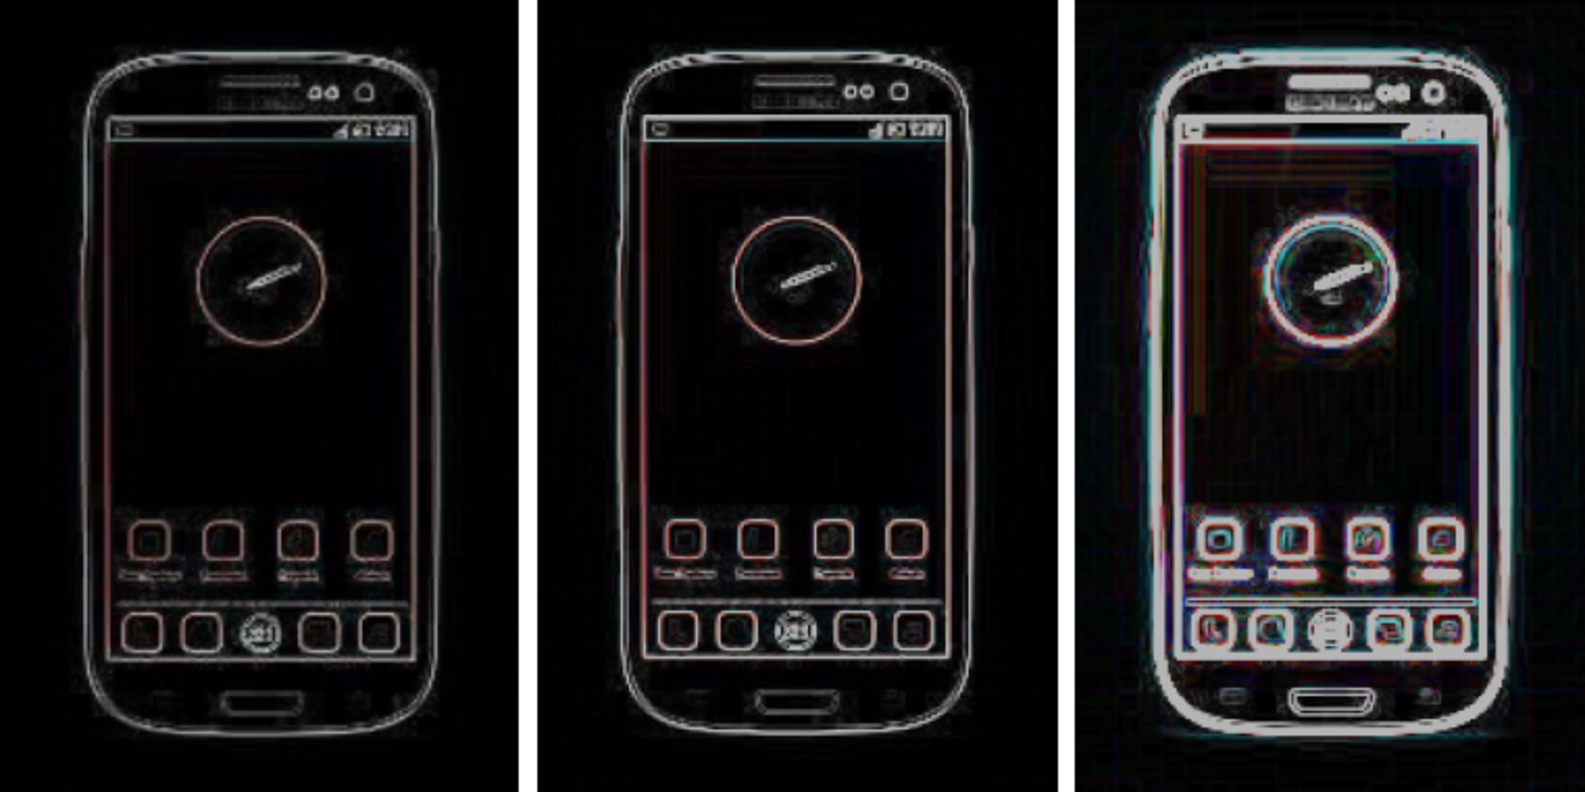
\includegraphics[width=\textwidth]{edge_detection_comparison}
	\caption[Comparison of the three edge-detection algorithms.]{Comparison of the three edge-detection algorithms. The left image is simple Gradient operators. At the middle its Roberts cross-gradient operators. The right image is for Sobel operators. Adapted from \cite{Fonseca2017_acondicionamento_imagem}}
	\label{fig:edge_detection_comparison}
\end{figure}

% subsubsection image_segmentation_edge_detection

\subsubsection*{Histogram}
\label{subsubsec:image_segmentation_histogram}

An Histogram is a graphical representation of the distribution of pixel intensities. It can be represented as a bar chart where each bin represents one pixel intensity or an interval. To create the histogram, each pixel intensity is placed on the right bucket according to its value (see Fig. \ref{fig:histogram}).

\begin{figure}[htbp]
	\centering
	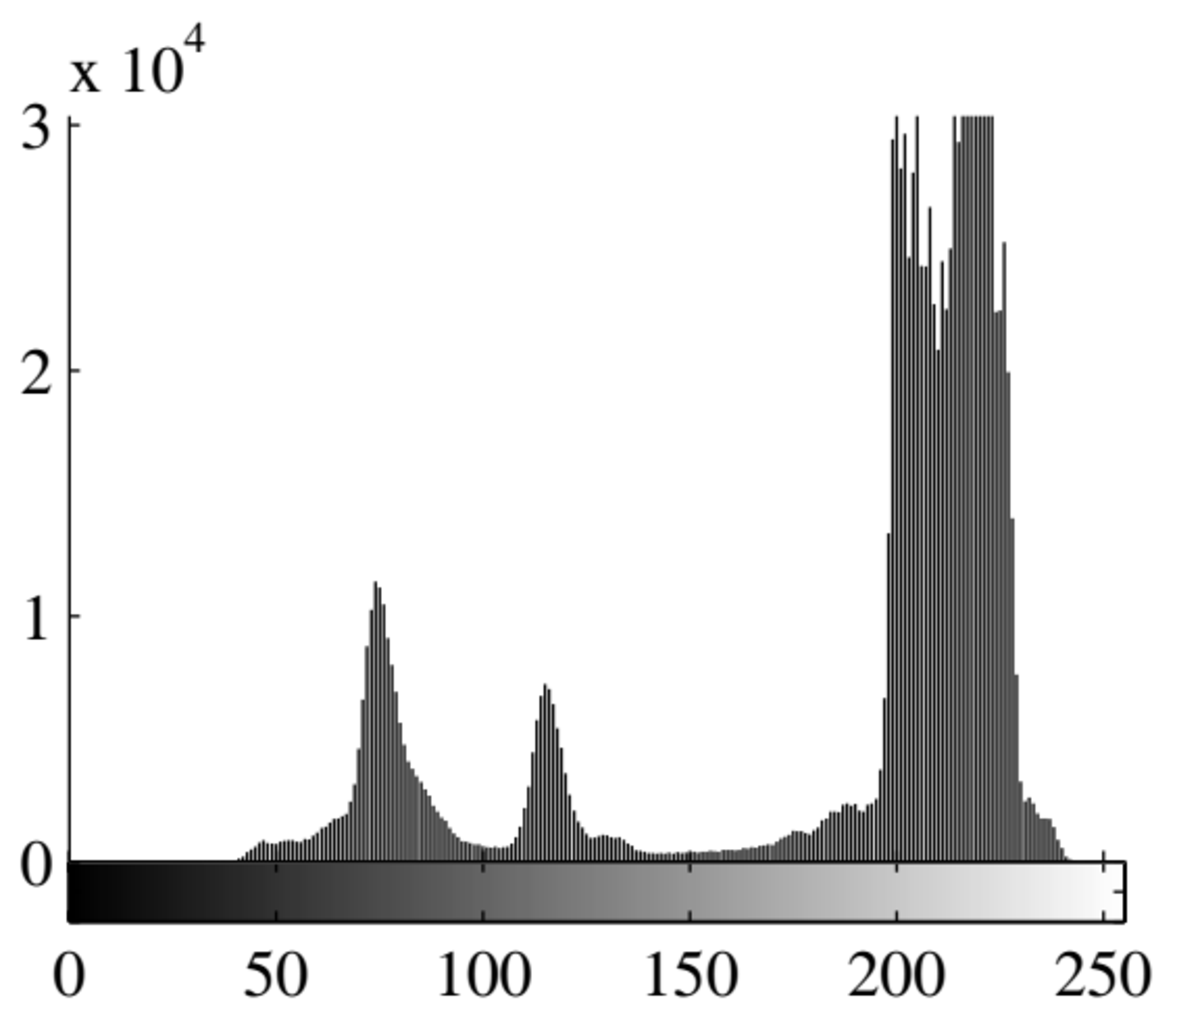
\includegraphics[width=.5\textwidth]{histogram}
	\caption[Histogram from a grayscale image.]{Histogram from a grayscale image. The y-axis represents the pixel count and the x-axis the pixel intensities from 0 to 255.}
	\label{fig:histogram}
\end{figure}

An histogram can be used to select the threshold value for image binarization like in the Otsu algorithm. It can also be used to create a binary mask that segments part of an image for background replacement. This technique is used on the movie industry with green screen technology (Fig. \ref{fig:histogram_binary_mask}).

\begin{figure}[htbp]
	\centering
	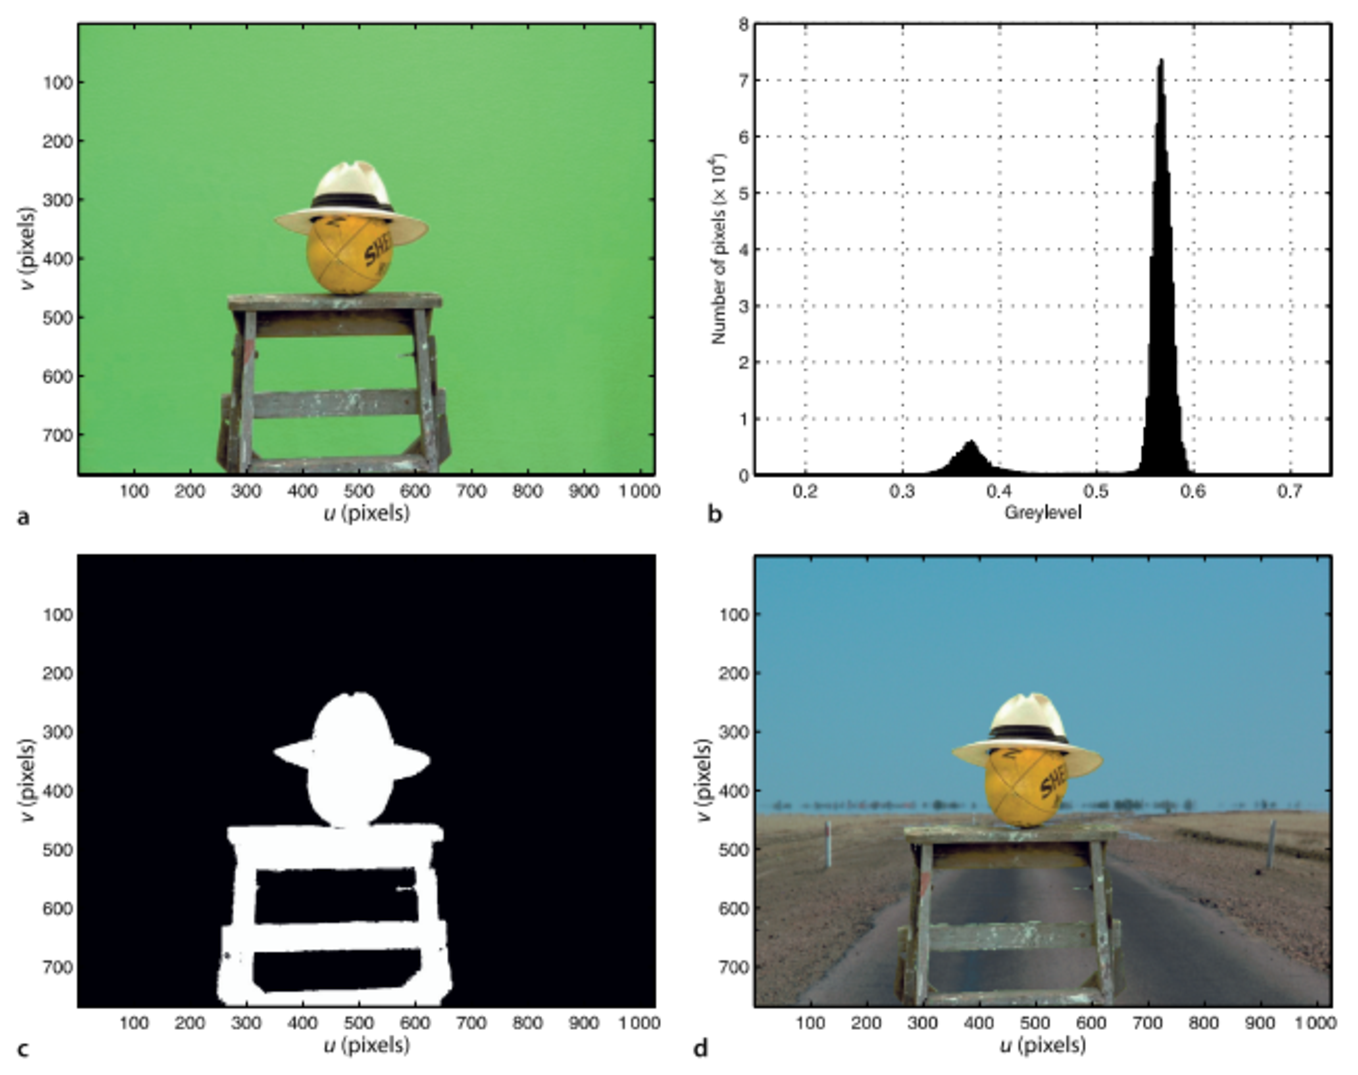
\includegraphics[width=\textwidth]{histogram_binary_mask}
	\caption[Chroma-keying.]{Chroma-keying. (a) The subject against a green background; (b) a histogram of green chromaticity values; (c) the computed mask image where true is white; (d) the subject masked into
a background scene. \cite{Corke2011_robotics_vision_control}}
	\label{fig:histogram_binary_mask}
\end{figure}

% subsubsection image_segmentation_histogram

% subsection image_segmentation

% = Stereo cameras =
\subsection{Stereo cameras}
\label{subsec:stereo_cameras}

Stereo cameras, also callled depth cameras, are dual-camera systems that mimic the human binocular vision. Binocular vision produces three dimensional information by comparing two vantage points. Depth is calculated by estimating disparities between matching key points on both images (Fig. \ref{fig:stereo_vision_diagram}).

\begin{figure}[htbp]
	\centering
	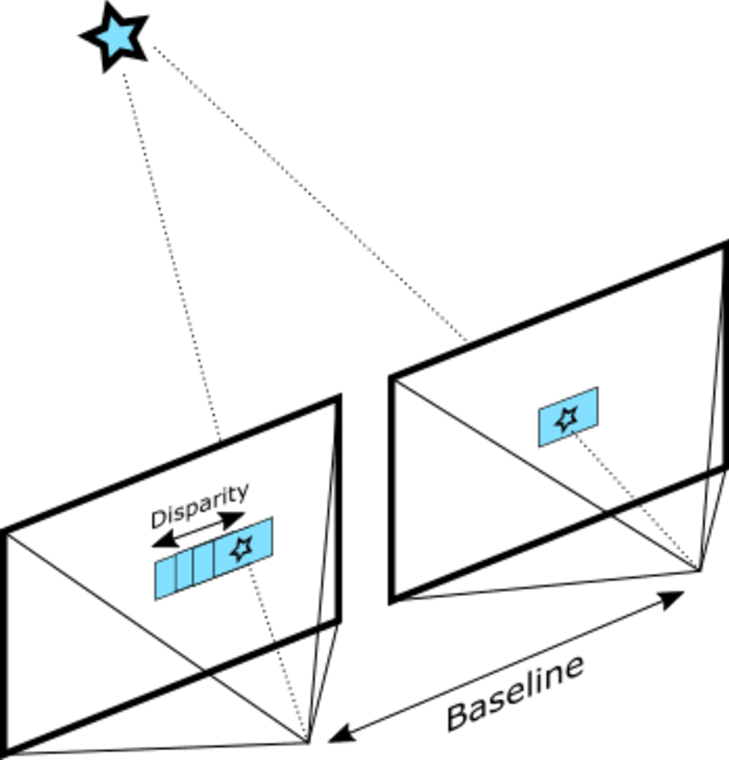
\includegraphics[width=.5\textwidth]{stereo_vision_diagram}
	\caption[Depth from stereo algorithm finds disparity by matching blocks in left and right images.]{Depth from stereo algorithm finds disparity by matching blocks in left and right images. Adapted from \cite{IntelRealSense_basics_depth_vision}}
	\label{fig:stereo_vision_diagram}
\end{figure}

The main algorithm to produce a depth map from binocular vision is called triangulation. Figure \ref{fig:depth_from_stereo_triangulation} presents the problem setup. From the geometry rules of similar triangles, it can be noticed that

\begin{equation}
    \label{eq:stereo_vision_triangulation_equations}
    \frac{z}{f} = \frac{x}{x_l} \quad,\quad \frac{z}{f} = \frac{x-b}{x_r} \quad,\quad \frac{z}{f} = \frac{y}{y_l} = \frac{y}{y_r}.
\end{equation}

\begin{figure}[htbp]
	\centering
	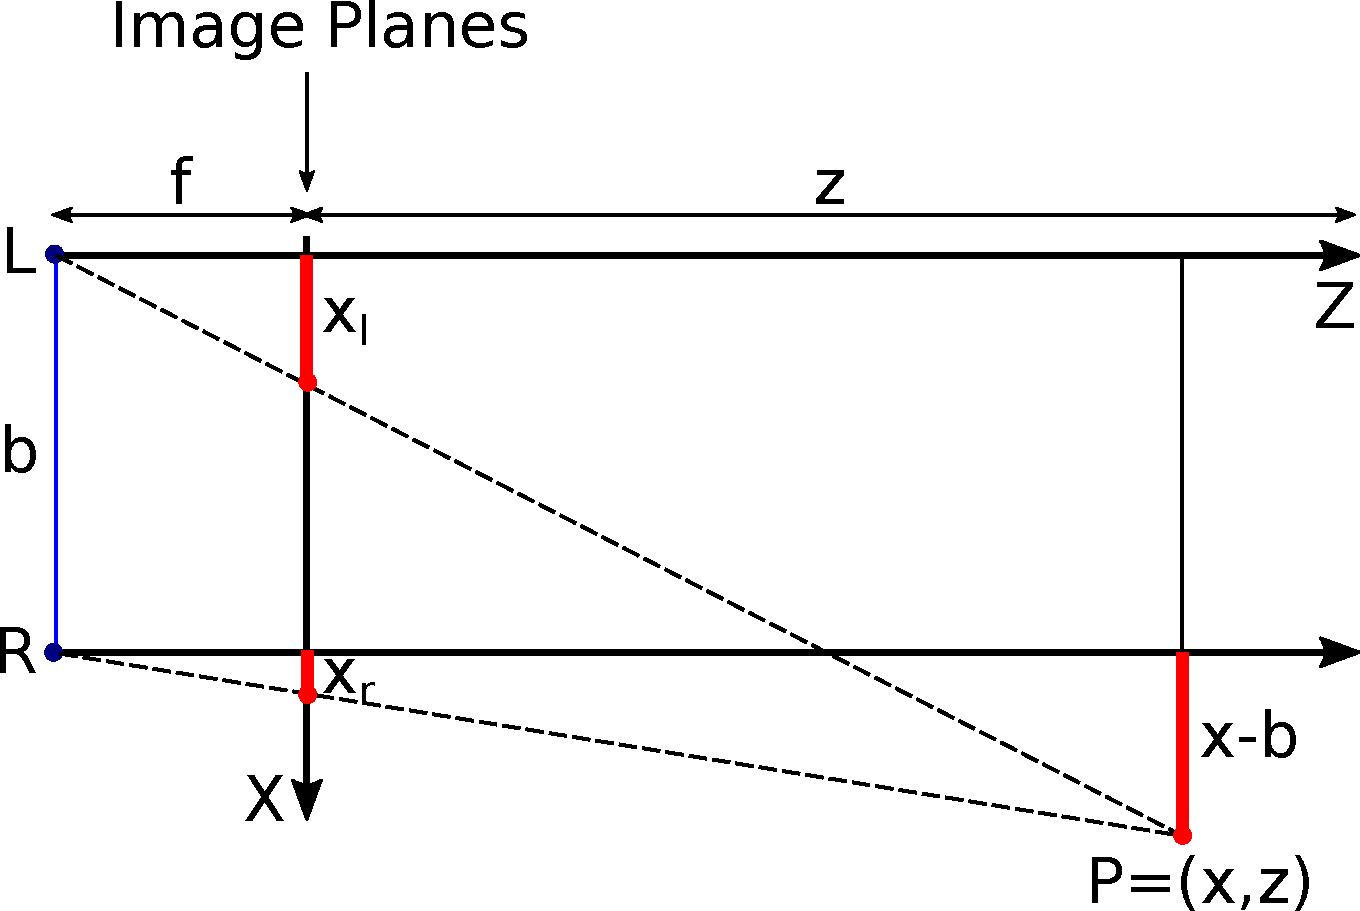
\includegraphics[width=.8\textwidth]{depth_from_stereo_triangulation}
	\caption[Triangulation for depth calculation from stereo cameras.]{Triangulation for depth calculation from stereo cameras. $L$ and $R$ are the left and right cameras positions, respectively. The distance $b$ between them is the baseline. $x_l$/$x_r$ are the distances between the left/right optical axis and the intersection point of the line of sight with the image planes. $f$ is the cameras focal length. The y-axis is perpendicular to the page. Adapted from \cite{Rao2009_stereo_3d_vision}}
	\label{fig:depth_from_stereo_triangulation}
\end{figure}

"For stereo cameras with parallel optical axes, focal length $f$, baseline $b$, corresponding image points ($x_l$,$y_l$) and ($x_r$,$y_r$)" \cite{Rao2009_stereo_3d_vision}, the location of the 3D point can be derived from equations (\ref{eq:stereo_vision_triangulation_equations}), and corresponds to the following

\begin{equation}
    \left\{
    \begin{aligned}
    & z = \frac{f \cdot b}{x_l - x_r} = \frac{f \cdot b}{d} \\
    & x = \frac{x_l \cdot z}{f} = b + \frac{x_r \cdot z}{f} \\
    & y = \frac{y_l \cdot z}{f} = \frac{y_r \cdot z}{f}
    \end{aligned}
    \right.
    \quad,
\end{equation}

where $d$ is called the disparity and is equal to $x_l - x_r$.

The main problem of this procedure is that it depends on finding the correspondence between the same point on both projections. The most naive algorithm to find this correspondence is the \glsfirst{ssd}. The depth map obtained is an image where each area or pixel has a value corresponding to its depth (Fig. \ref{fig:ssd_stereo_vision_results}). From this information it is possible to create a point cloud.

\begin{figure}[htbp]
	\centering
	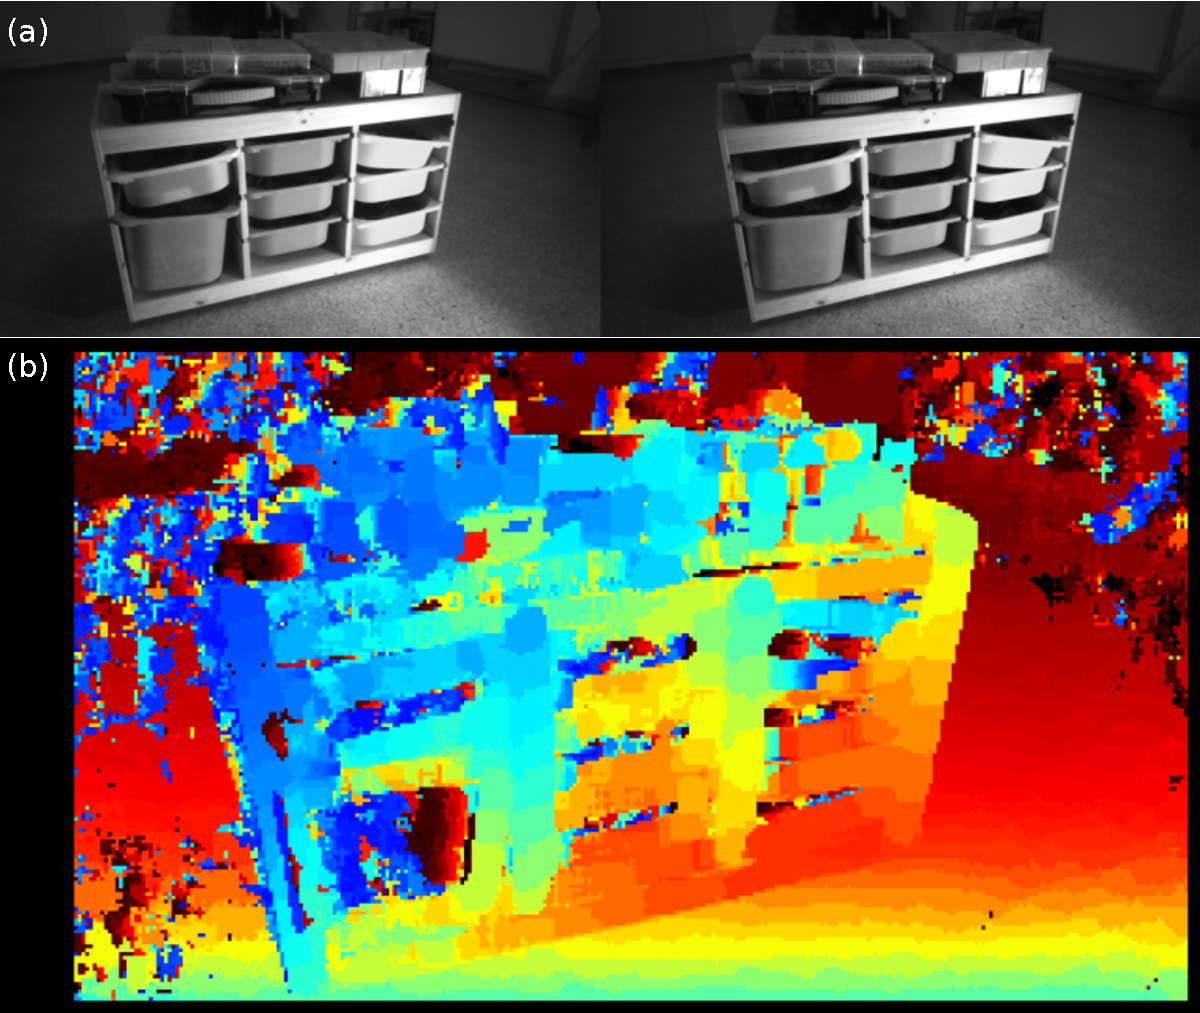
\includegraphics[width=.8\textwidth]{ssd_stereo_vision_results}
	\caption[Results from the \gls{ssd} algorithm.]{Results from the \gls{ssd} algorithm. (a) Stereo cameras source image. (b) Depth map obtained. The blues are closer to the camera and the reds further away. Adapted from \cite{IntelRealSense_basics_depth_vision}}
	\label{fig:ssd_stereo_vision_results}
\end{figure}

% subsection stereo_cameras

% = Point clouds =
\subsection{Point clouds}
\label{subsec:point_clouds}

A point cloud is a 3D data format consisting on a collection of points on 3D space. This data is generated by 3D scanners, range finders and depth cameras (Fig. \ref{fig:realsense_point_cloud}). Point clouds have many use cases. For example it is used to produce 3D CAD models, for metrology, animation, object detection, and more. Because each point has its three dimensional coordinates in relation to the cloud generator, it can be used to create surface meshes, estimate volumes and distances.

\begin{figure}[htbp]
	\centering
	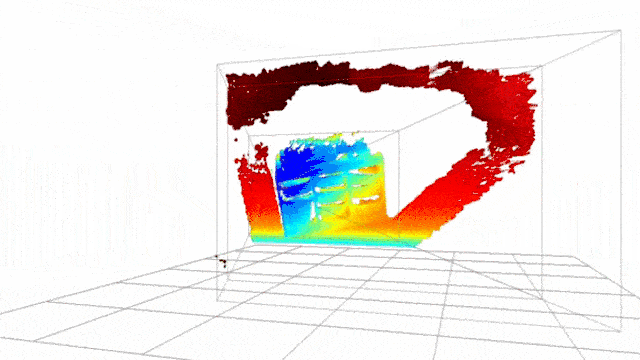
\includegraphics[width=\textwidth]{realsense_point_cloud.png}
	\caption[Point-cloud using Intel RealSense D415 stereo camera.]{Point-cloud using Intel RealSense D415 stereo camera. Adapted from \cite{IntelRealSense_basics_depth_vision}}
	\label{fig:realsense_point_cloud}
\end{figure}

% subsection point_clouds

% section computer_vision